\hypertarget{earlyexiting}{%
	\chapter{Early Exiting}\label{ch:earlyexit}}
\thispagestyle{fancy}

In this chapter we study accuracy latency trade-off of the early exiting \gls{dnn}s, by experimentation of exit thresholds and delay thresholds. We have found, that the early exiting have capabilities to better accommodate delay threshold, than conventional single-exit \gls{dnn}s. The chapter is structured as follows, in section\ref{sec:ee-branchy-vs-cascaded}   present the early exit proposals \gls{branchynet} ann Cascaded \gls{dnn}. In section \ref{sec:ee-metrics} we define the metrics used in our experiments. In section \ref{sec:ee-exp-setup} we descibe our experimental setup. In Section \ref{sec:ee-implementation} we describe the implementation details of our early exiting models B-\gls{resnet} and B-\gls{densenet}. In section \ref{sec:ee-results} we present our results of training the models and experimenting with the fast inference framework using exit threshold and delay threshold. In section \ref{sec:ee-summary} we discuss our results.

%Early exiting \gls{dnn} draws inspiration from another \gls{cv} algorithm, Viola-Jones \cite{viola_rapid_2001}. Viola Jones Face Detection was proposed in \citeyear{viola_rapid_2001}. The idea is a stacking or cascaded less accurate predictors to build a strong predictor. The predictors increasingly gain confidence when running the algorithm which termintates when the confidence has reached a threshold. Early exiting \gls{dnn} likewise stacks multiple classifiers. The \gls{dnn} can too be terminated, when a prediction with satisfying confidence is obtained. 



% and have primarily been used to solve two challenges in current literature.
%
%\begin{enumerate}
%	\item Reducing average inference latency and power consumption by letting samples prematurely exit the model based on a threshold measure of confidence \cite{teerapittayanon_branchynet:_2016}.
%	\item Comply with application time constraints by exit selection or sub-model selection. By only inference samples up to a selected exit possible to meet stringent delay constraints and reduce waste of computation \cite{li_edge_2018}. 
%\end{enumerate}

\section{BranchyNet vs. Cascaded DNN} \label{sec:ee-branchy-vs-cascaded}

\gls{branchynet} \cite{teerapittayanon_branchynet:_2016} and cascaded \gls{dnn} \cite{leroux_resource-constrained_2015} was published around the same time. We describe the two very similar proposals and how they differ.  Cascaded \gls{dnn} adds intermediate classifiers after a layer, or a block of layers in a \gls{dnn}, wheres \gls{branchynet} constructs early exit branches with additional layers, see figure \ref{fig:cascaded-vs-branchy}.

\begin{figure}
	\centering
	\subfloat[Branchy AlexNet, Source \citetitle{teerapittayanon_branchynet:_2016} \cite{teerapittayanon_branchynet:_2016}]{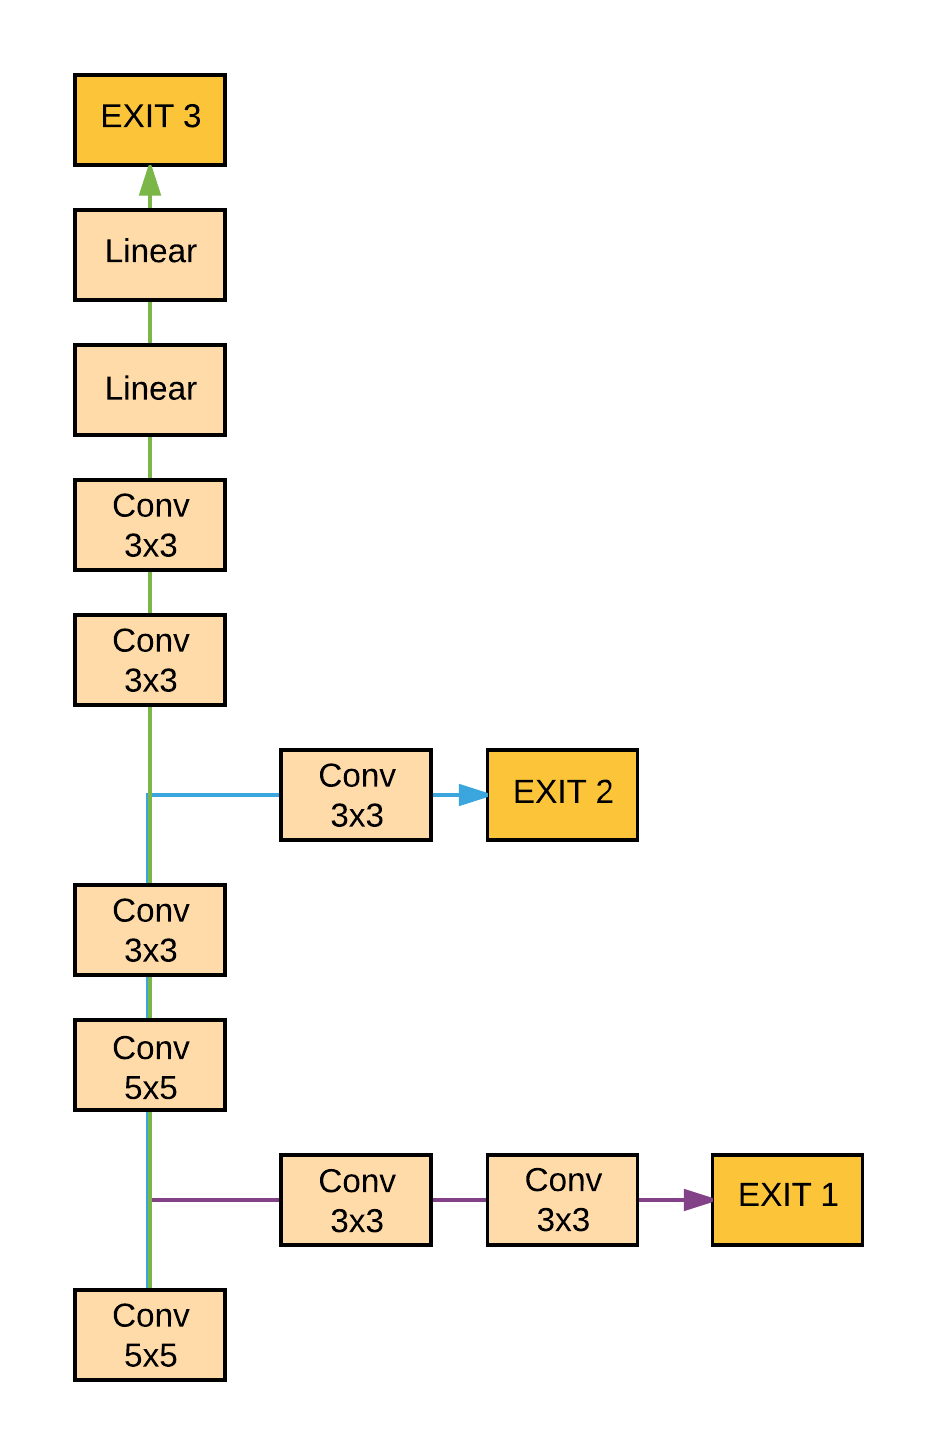
\includegraphics[height=.3\textheight]{figures/articles/branchynet}}
	\hspace{2em}
	\subfloat[Cascaded \gls{dnn}, Source \citetitle{leroux_resource-constrained_2015}\cite{leroux_resource-constrained_2015}]{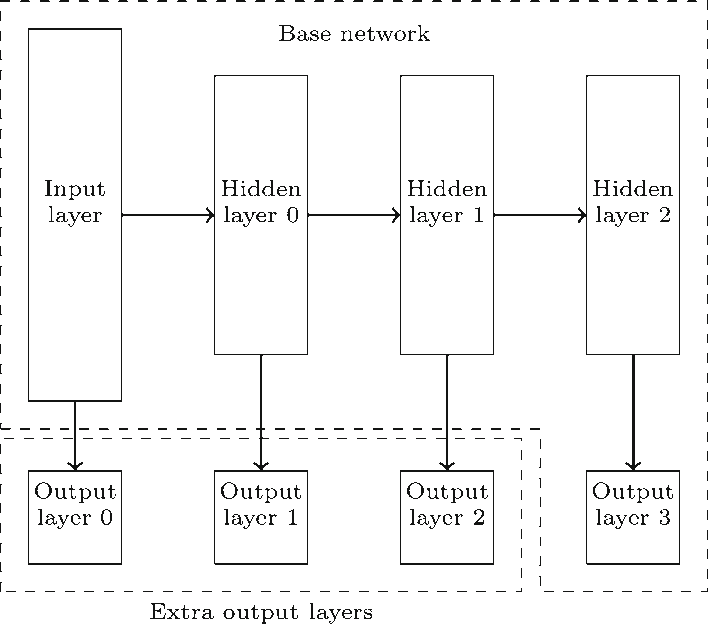
\includegraphics[height=.3\textheight]{figures/articles/cascade_dnn}}
	\caption[\gls{branchynet} vs. Cascaded \gls{dnn}]{\gls{branchynet} vs. Cascaded \gls{dnn}}
	\label{fig:cascaded-vs-branchy}
\end{figure}

Early exiting relies on the assumption, that the majority of samples are easy to classify correctly, and that \gls{dnn}s only have become deeper to accurately classify more difficult samples. As figures \ref{fig:hardvseasydog} exemplifies, samples where the object is easily separated from the background, are not occluded, and are viewed from angles which makes it easier to classify. Contrary samples that are not, are harder, additionally if the sample, should be discriminated from classes, with similar features are difficult such as different dog breeds etc. These examples have been found by running an early exit model. The hard examples have been found from looking at samples, that the \gls{dnn}s failed to classify, or can only classify using the last exit. The easy example are found by looking at samples, that can be correctly classified with high confidence by the first exit. 

\begin{figure}
	\captionsetup[subfigure]{justification=centering}
	\centering
	\subfloat[bluetick]{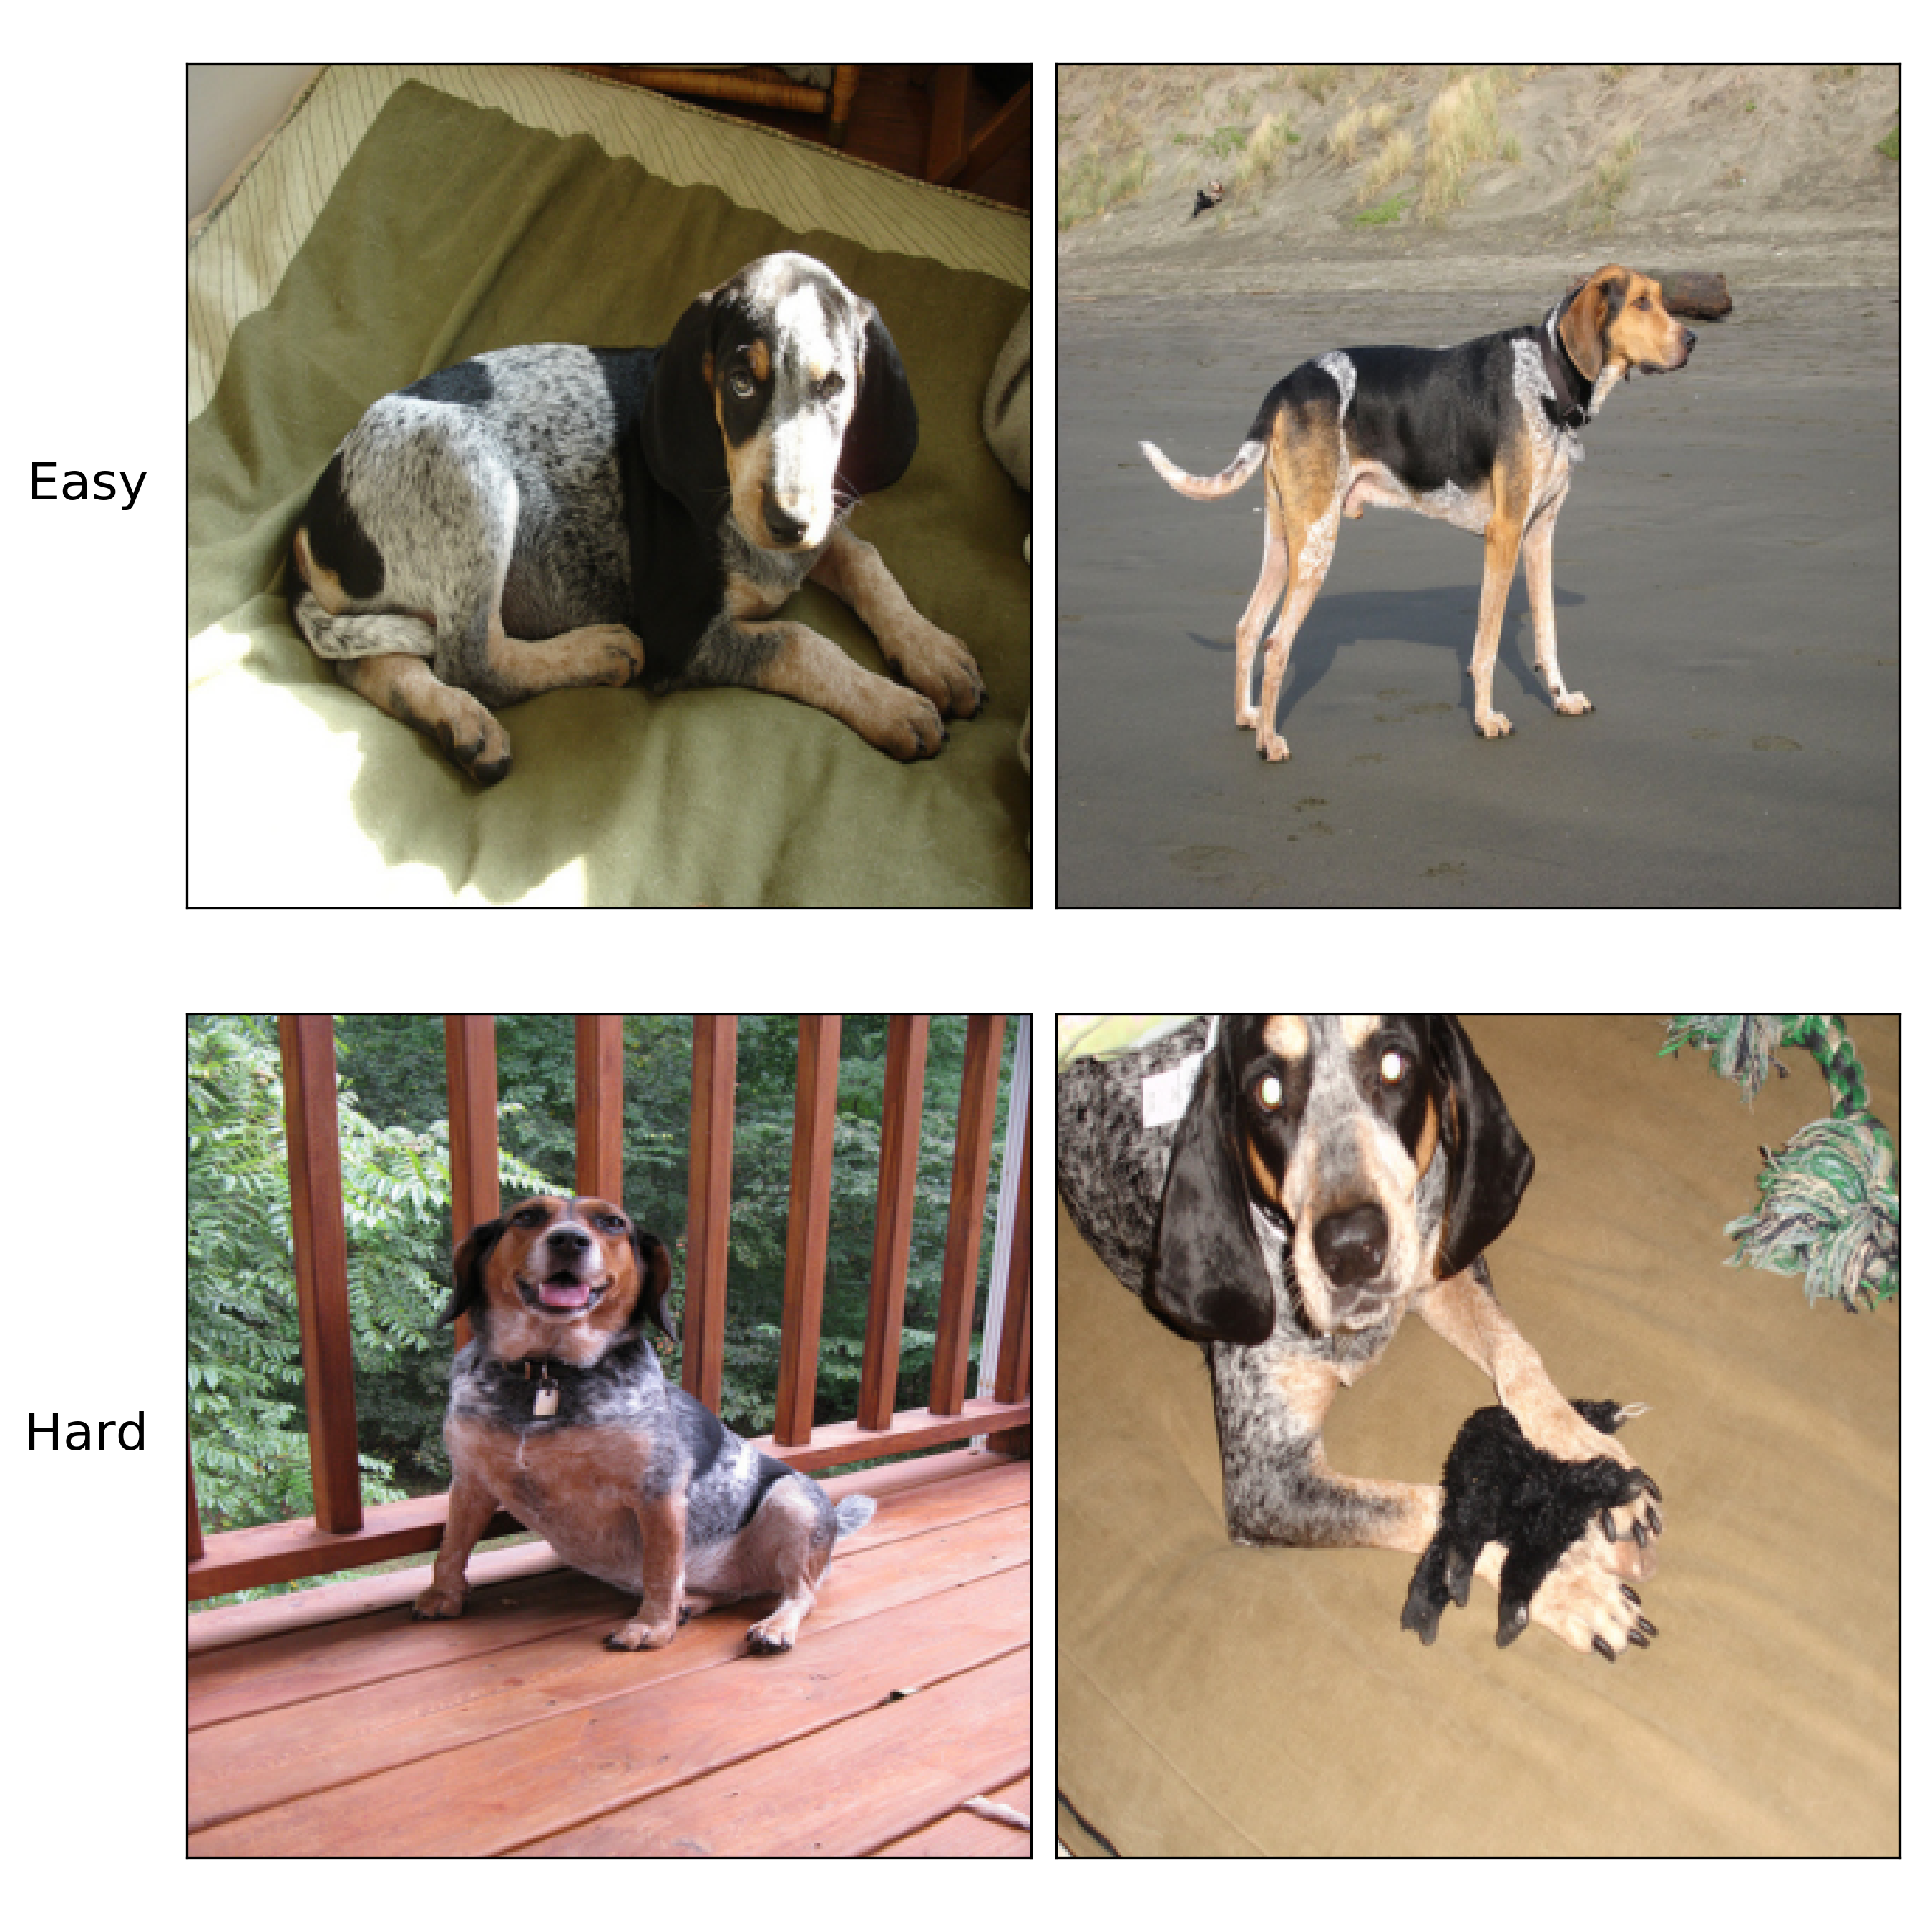
\includegraphics[width=0.5\linewidth]{figures/illustrations/hard_vs_easy_dog}}
	\subfloat[flamingo]{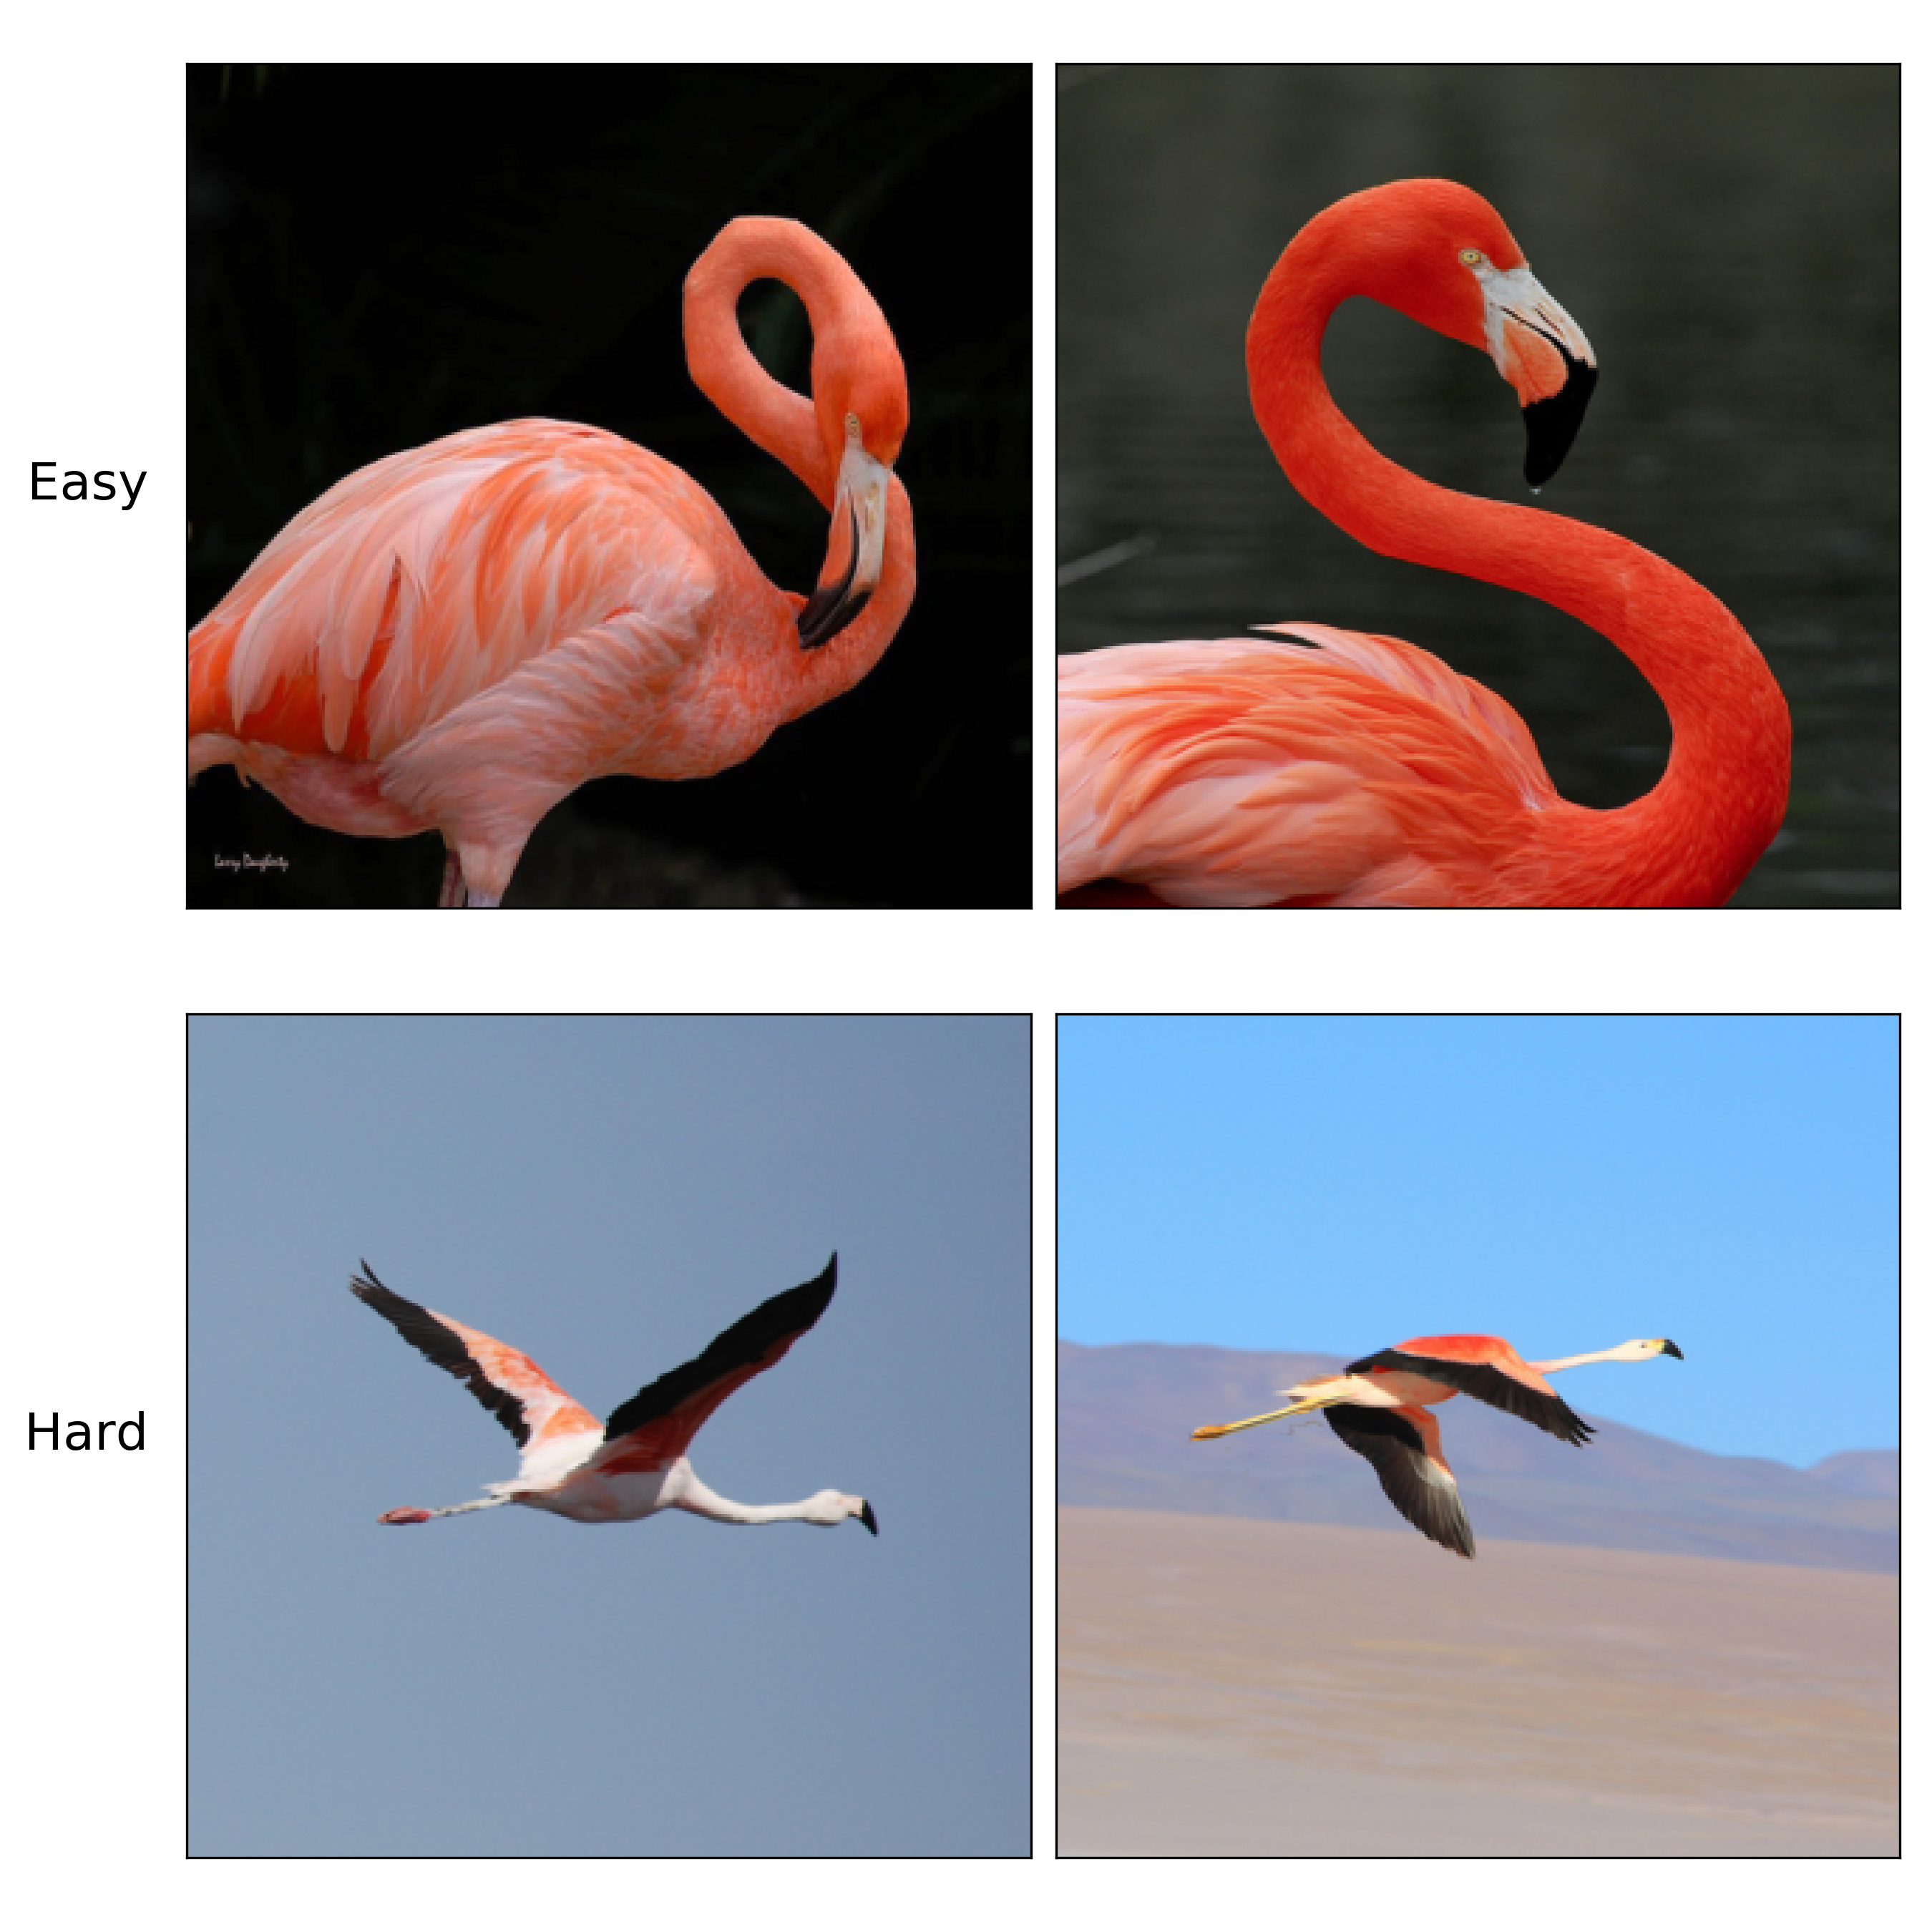
\includegraphics[width=0.5\linewidth]{figures/illustrations/hard_vs_easy_flamingo}}
	\caption[Easy vs. Hard Samples]{Easy vs. Hard Samples}
	\label{fig:hardvseasydog}
\end{figure}

\paragraph{Fast Inference Framework} The inference framework for the two proposal \gls{branchynet} and Cascaded \gls{dnn} are almost identical. A sample is inferred up to an exit and based on an exit criteria, it is decided to exit or to continue the inference. The only difference is the choice of exit threshold. Cascaded \gls{dnn} uses the softmax score of the prediction, and evaluates if the score higher than a selected threshold, it is exited. \gls{branchynet} determines the entropy of the softmax output, and evaluates if the entropy is less than a selected threshold, the sample is is is exited.

The algorithm we use for early exit fast inference is provided in listing \ref{lst:score-margin-inference}. Note the algorithm uses the confidence threshold for exit decision.

\begin{minipage}{\linewidth}
	\begin{lstlisting}[language = {}, mathescape=true, caption={Early Exit using Score-margin }, label={lst:score-margin-inference}]
procedure $\textsc{EarlyExitFastInference}$$(x, T )$
	for $k = 1\dots K$ do
		$z = f_{exit_k}(x)$
		$ \hat{y} = softmax(z) $
		if $\hat{y} > T_k$ then
			return $\arg \max \hat{y}$
	return $\arg \max \hat{y}$ 
	\end{lstlisting}
\end{minipage}

Early exiting have shown promising result in other works. In \cite{berestizshevsky_sacrificing_2019}, they suggest removing convolutional layers of branches in \gls{branchynet}, to reduce the amount of branch computation. They show a 2 $ \times $ speed-up at only the cost of 1 \% accuracy using two fully-connected layers in exits.

In \cite{kaya_shallow-deep_nodate}, \emph{Overthinking}, the phenomena where an early exit correctly classifies an input, but a later exit makes it wrong is investigated. They propose to use the highest scoring prediction from all exits to cope with overthinking. 

\paragraph{Training Framework} 
Training cascaded \gls{dnn}, in \cite{leroux_resource-constrained_2015} it is proposed to train a network using a single end-classifier. Once the model has reaches convergence, the intermediate classfiers are attached and the entire network is trained for one single epoch, before freezing the network weights and training the classifiers. This is equivalent to use a pre-trained model and convert it to a cascaded model. The approach was tested and gave unsatisfactory results, see figure \ref{fig:frozen-b-resnet-miniimagenet-100}. In \cite{leroux_cascading_2017}, the follow-up paper to cascaded \gls{dnn}, they too train a frozen base network on the ImageNet dataset, but does not achieve better performance for early exit classifiers.  

The \gls{branchynet} approach is remarkably similar. In \cite{teerapittayanon_branchynet:_2016} they define the \gls{branchynet} loss function, as an extension of the widely used softmax cross-entropy loss function.
\begin{align}
L\left(\mathbf{y},\hat{\mathbf{y}}\right) = - \frac{1}{C} \sum_{j =1}^{C} y_c \log \hat{y}_c
\end{align}
Where $ \bm{y} $ is a on-hot encoded ground truth vector, $ \bm{\hat{y}} $ is the output score vector of the softmax classfier and $ C $ is the number of classes and $ c \in \left[1, C\right] $ is the class labels.
	
The \gls{branchynet} loss function is defined as the weighted sum of the softmax cross-entropy loss of each branch-prediction. 

\begin{align}
	L_{\mathrm{BranchyNet}}(\hat{\mathbf{y}},\mathbf{y};\theta) = \sum_{n=1}^{N} w_n L \left(\hat{\mathbf{y}}_{n},\mathbf{y};\theta\right)
\end{align}

Where $ \bm{\hat{y}} $ is the output score vector of exit $ n $, $ w_n $ is the weight for exit $ n $ and $ \theta $ represents the parameters of the layers from an entry point to the exit point $ n $.

They claim, that the joint-optimization of multiple exits provides a regularization effect, thus countering over-fitting and potentially improves test accuracy. Additionally is also mitigates vanishing gradient, due to additional gradient signal from the early exits, which promotes more discriminative feature in early layers. In \gls{googlenet} \cite{szegedy_going_2015} auxiliary classifiers are too place in the middle of the network to counter vanishing gradients. However, that is also the only purpose of the auxiliary classifiers, as they are only used when training the network. Thus, no samples can exit the inference process prematurely. 

In \gls{branchynet}, they have also too found, that first training the network end-to-end or using a pre-trained model, and then attach the intermediate exits/classifiers both improves the performance and shortens the training time, as in cascaded \gls{dnn}. However, they do not suggest to freeze the features of the base model, but to train the entire model. We have tried both freezing and unfreezing the network base and have found, that training the entire model is the far superior approach, see figure \ref{fig:b-resnet-miniimagenet-100}. 

In the next section we explain the \gls{msdnet} \cite{huang_multi-scale_2017}, a novel \gls{dnn} specifically designed for early exits.

\section{Multi-Scale Dense Network}

A study in \cite{huang_densely_2016} show that densely connected layers of \gls{densenet} are more suitable for early exiting, than the popular \gls{resnet} architecture build of residual blocks. Densely connected block uses a concatenation of features from all layers for final classification. The combination of  general feature and increasingly more specific and complex features are shown to be important for early exiting models. This finding have been used to come of the novel \gls{dnn} design. A further elaboration of the network layers are found in section \ref{sec:ee-implementation}. Figure \ref{fig:msdnet} from the original article Multi-scale path on the vertical axis and the depth on the horizontal axis. The figure show the stacking of filters that are concatenated (c) along both axes. Each block contain an exit with a classifier.

\begin{figure}
	\centering
	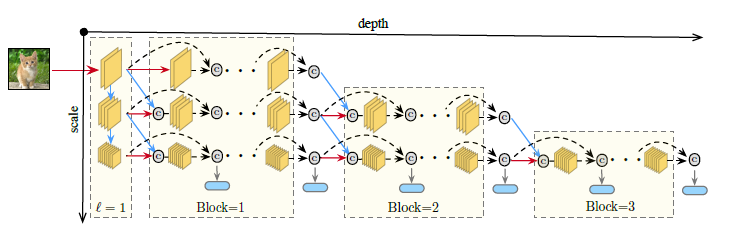
\includegraphics[width=\linewidth]{figures/models/msdnet}
	\caption[\gls{msdnet} Architecture]{\gls{msdnet} Architecture, Source: \citetitle{huang_multi-scale_2017} \cite{huang_multi-scale_2017}}
	\label{fig:msdnet}
\end{figure}

The work addresses two main problems concerning early exiting. The first problem is the lack of coarse-level features in early classifiers. Traditional \gls{dnn}s uses stacking of layers to get coarse level features, which the early classifier lacks, thus giving unsatisfactory high error-rates. Multi-scale feature maps addresses this issues by preserving high-resolution information and allow constructing coarse-level features for all classifiers in the network.

The second problem is early classifiers interfere with later classifiers. The early classifiers might cause early features to be optimized for the short-term by collapsing information prematurely, thus harming the later and final classifiers. Their study reveals, that densely connected layers suffers much less from intermediate classifiers than residual layers, as a layer is connected to all previous layer and is therefore able to recover collapsed information. We elaborate upon the two different types of layers in section \ref{sec:ee-implementation}. We experiment with \gls{resnet}, \gls{densenet} and \gls{msdnet} in our experiments.

In the next section we describe the mathematical models used to evaluate the latency, accuracy and early exiting capabilities using confidence and delay thresholds.

\section{Analytical Model} \label{sec:ee-metrics}

Assume $ C $ denotes the number of image classes, $ N $ denotes the number of the exit points in a DNN, $ I $ denotes the number of images.

	\begin{enumdescript}
		\item[Inference Latency] is defined as the time for a \gls{dnn} to provide a prediction. 
		
		\begin{minipage}[t]{\linewidth}
			\captionof{figure}[\gls{dnn} structure and latency]{\gls{dnn} structure and latency}
		\end{minipage}
		
		\gls{dnn}s are build of blocks and classifiers. We adapt the same notation for the early exiting inference model and the conventional inference model with a single exit at the end of the \gls{dnn}. 
		
		Assume:
		\begin{itemize}
			\item $T_{i,n}^{block}$ denotes the runtime inference an image $ i $ to the $ n $th block of the \gls{dnn} $ i $ for $ \left(1\leq n \leq N, 1 \leq i \leq I\right) $
			\item $T_{i,n}^{exit}$ denotes the runtime of the exit $ n $  to process image $i$ for $ \left(1\leq n \leq N, 1 \leq i \leq I\right) $
		\end{itemize}
		\begin{enumdescript}
			\item[Conventional Inference Latency] The conventional inference model only have a single exit at block $ N $, hence all $ N $ blocks of the \gls{dnn} must have inferred the image $ i $ before $ i $ i classified at exit $ N $. Thus the latency model for a conventional inference model is presented as
			\begin{align}
			T^{ci}_{i}= \sum_{j=1}^{N} T_{i,n}^{block} + T_{i,N}^{exit}
			\end{align}
			\item[Early Exit Inference Latency] The early exit inference model is adaptive. The inference of image $ i $ can terminate at any exit $ n $. If the classification exits from exit point $ n $, then the latency model for early exit inference model is presented as
			\begin{align}
			T_{i,n}^{ee}=\sum_{j=1}^{n} \left(T_{i,n}^{block} + T_{i,n}^{exit} \right) 
			\end{align}
			The additional classifiers of the early exit inference model add a overhead compared to the conventional inference model, however it may not be required to run all $ n $ blocks and classifiers of the early exiting inference model. 
		\end{enumdescript}
		
		\item[Classification Accuracy] is the defined as the fraction of correctly classified samples out of all samples. The inference accuracy of exit point $ n $ can be expressed by
		\begin{align}
		\bar{A}_{n}=1-\frac{1}{I} \sum_{i=1}^{I} \mathbb{I}\left(\left|\hat{c}^*_{i,n}-c_{i}\right|\right) \label{eq:accuracy}
		\end{align}
		%We can express the ground truth as a one-hot encoded vector $ \bm{y}_i $
		where the ground truth class label of image $ i $ and $ c_i \in \left[1, C \right] $ and $ \mathbb{I(\cdot)}  $ is a indicating function defined by
		\begin{align}
		\mathbb{I}(a)= \begin{cases}
		0, & \mathrm{if\:} a \leq 0, \\
		1, & \mathrm{otherwise}
		\end{cases}
		\end{align}
		    		
		Note for the conventional model only a single $ A_N $ can be expressed, as the model only has a single exit.
		
		The prediction output from the softmax classifier is denoted
		\begin{align}
			\mathbf{\hat{y}}_{i,n} = \left[\begin{array}{ccccc}\hat{y}_{i,n,1} & \hat{y}_{i,n,2} & \hat{y}_{i,n,c} & \dots & \hat{y}_{i,n,C}\end{array}\right]
		\end{align}
		Where $ \hat{y}_{i,n,c} $ denotes the score of class $ c $ from exit point $ n $ by processing image $ i $
		
		The prediction is the highest scoring class of the softmax output. The class label of the prediction is denoted $ \hat{c}^*_{i,n} $ and is expressed as
		\begin{align}
		\hat{c}^*_{i,n} = \arg \underset{c}{\max}\: \mathbf{\hat{y}}_{i,n}
		\end{align}
		The score associated the class label is of image $ i $ from the exit point $ n $ is
		\begin{align}
		\hat{y}^*_{i,n} = \underset{c}{\max}\: \mathbf{\hat{y}}_{i,n}
		\end{align}
	
		Note that the prediction to go through the entire \gls{dnn} is $ \bm{\hat{c}}^*_i  = \arg \underset{c}{\max} \bm{\hat{y}}_{i,N} $, i.e. the last exit $ N $ of the early exit model, or equivalent to the prediction of conventional inference model.
  
		\item[Early Exit Condition] we define the early exit condition based on the output of our scoring function $ f_\phi(\bm{\hat{y}}_{i,n}) $, given the score vector $ \bm{\hat{y}}_{i,n} $ for image $ i $ at exit point $ n $. An image $ i $ is allowed to exit the model at exit point $ n $, if a score threshold $ \gamma $ is surpassed. 
		
		We assume $	\gamma \in \left[0,1\right] $, as the all scores of  $ \bm{\hat{y}}_{i,n} $ sum to 1. Note that, although the score threshold could be different from exit points, in our experiments, we use the same threshold, since we are concerned with the latency. Selecting a higher threshold value at an early exit, will cause less samples to exit and promote use of later exits, which will cause additional inference delay. It is seen in \cite{teerapittayanon_finding_2018}, that finding different threshold values for the exits can improve the accuracy.
		
		We express the probability of early exit at exit $ n $, given the score function. 
		\begin{align}
		\overline{F}^{exit}_n = \frac{1}{I}\sum_{i=1}^{I} \mathbb{I} \left(\gamma-f_{\phi}\left(\bm{\hat{y}}_{i,n}\right) \right)
		\end{align}
		
		Where $ f_\phi\left(\bm{\hat{y}}_{i,n}\right) $ is a scoring function and for notation simplicity we write 
		\begin{align}
			f_{\phi}\left(\bm{\hat{y}}_{i,n}\right) = \begin{cases}
			 	f_{max}\left(\bm{\hat{y}}_{i,n}\right)\\
			 	f_{margin}\left(\bm{\hat{y}}_{i,n}\right)
			\end{cases}
		\end{align}
		which means we can choose to use either one.
		
		We define two different score functions, the score-max $ f_{max}(\cdot) $ and the score-margin $ f_{margin}(\cdot) $. 
		
		\begin{enumdescript}
			
			
			\item[Score-Max] the score-max function $ f_{max}(\cdot)$ also used in \cite{leroux_resource-constrained_2015}, is a simple function, that takes the score vector $ \bm{\hat{y}}_{i,n} $ of image $ i $ at exit $ n $ as input and outputs the maximum value of the vector. We express it as 
			\begin{align}
			f_{max}\left(\bm{\hat{y}}_{i,n}\right) = \underset{c}{\max} \bm{\hat{y}}_{i,n}
			\end{align}
			\item[Score-Margin] the score-margin function $ f_{margin}(\cdot)$, is defined and used in \cite{park_big/little_2015}. The function also takes the $ \bm{\hat{y}}_{i,n} $ as input and returns the difference between the two largest elements. We express it as
			\begin{align}
			f_{margin}\left(\bm{\hat{y}}_{i,n}\right) = \hat{y}_{i,n}^{1st} - \hat{y}_{i,n}^{2nd}
			\end{align}
			where $ \hat{y}_{i,k}^{1st} $ denotes the largest element of $ \bm{\hat{y}}_{i,n} $ 
			and $ \hat{y}_{i,n}^{2nd} $ the second largest element of $ \bm{\hat{y}}_{i,n} $.
			
		\end{enumdescript}
	
	\item[Reliability] our main concern is time-critical application. We define the reliability as the fraction of samples, that con be correctly classified given a latency threshold $ \delta $.
	
	\begin{align}
	R= \bar{A} \cdot (1-\overline{F}^{to})
	\end{align}
	
	The timeout probability $ \overline{F}^{to} $ is defined as the number of samples not able to meet the delay requirement out of all samples in the set.
	\begin{align}
	\overline{F}^{to}=\frac{1}{I}\sum_{i=1}^{I} \mathbb{I}\left(T_{i}^{cmp}-\delta\right)
	\end{align}
	Where $ T_{i}^{cmp} $ denotes computation time irregardless of conventional inference model with a single exit, or early exit models with multiple. We only have a delay violation if $ T_i^{cmp} \leq \delta $, i.e. the model have not provided a single prediction within the time frame. Thus, if no exit of the model can meet the delay requirements and a prediction cannot be acquired, it is treated as a misclassification. 
		
	\item[Problem formulation] we select exit point for each image and optimize its accuracy with a latency constraint. The inference time of image $ i $ at exit $ n $, cannot be greater than or equal to our latency threshold $ \delta $. 
	
	\begin{maxi}
		{n}{\bar{A}_{n}}
		{}{}
		\addConstraint{T_{i,n}}{\leq \delta}
	\end{maxi}
%	where $\vec{n} = \left[n_1,,n_2, \dots, n_I\right]$. 
	
	To solve this problem, instead of making decision before processing the image, we simply use the best effort way, i.e., feed each exit results back and let user decide the prediction. For three reasons:
	\begin{enumerate}
		\item latency uncertainty make it hard to make decision in advance
		\item algorithm to make decision may take time
		\item going through classifier of each exit point would not take too long time.
	\end{enumerate}
		
	\end{enumdescript}


In the next section is the implementation of our B-\gls{resnet} and B-\gls{densenet} explained.


\section{Implementation} \label{sec:ee-implementation}

\subsection{Branchy-ResNet} 

In this section is the residual layers, the building block of the residual network, is explained. Followed by a design description of Branchy-\gls{resnet}.

The depth of \gls{dnn} is of paramount importance to extract increasingly richer features from images to obtain highly accurate classification models cite{who}. Training very deep models with more than ten layer for convergence is not easy due to vanishing/exploding gradients. Residual Networks or \gls{resnet} \cite{he_deep_2015} have for long been a state-of-the-art network and won ILSVRC15 using 152 layers. The network is build of residual blocks, a \gls{dnn} layer designed for extremely deep networks. 

Just as plain \gls{vgg} nets, residual networks is still a stacking of convolutional layers. The \gls{resnet}, however, adds a shortcut connection, which skips a layer or a block of layers. The skip connection adds the identity of input to the output of the layers/block, see figure \ref{fig:residualblock}

\begin{figure}
	\centering
	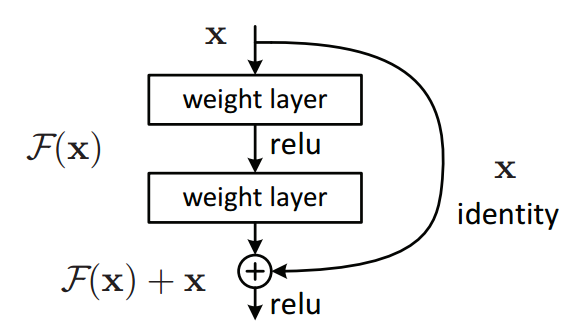
\includegraphics[width=.5\linewidth]{figures/models/residualblock}
	\caption[Residual Block]{Residaul Block}
	\label{fig:residualblock}
\end{figure}

Information from earlier layers are preserved by the residual, which diminishes the vanishing gradient problem. Thus this type of network have shown to be easier to train compared to it’s plain counterpart and able to obtain far superior accuracy.  

Very deep residual networks comprised of up to 152 layers have also shown to be far more efficient requiring less \gls{flop}s, than \gls{vgg}16 comprised of only 16 layers, by introducing a bottleneck unit. The bottleneck reduces the dimensions, applies the concolutional filters, and then restores the dimensions.

The residual networks proposed in \cite{he_deep_2015} are grouped into 4 resolutions block each of which downsamples the input data. The network are proposed with different number of layers (18, 34, 50, 101, 152) exemplifying th ability to train extremely deep networks. Table \ref{tbl:resnet101} describes the blocks and layers of the \gls{resnet} architecture. \gls{pytorch} provide implementations of these networks. The implementations can be trained from scratch or can be initialized with downloadable pretrained weights based on ImageNet. \gls{resnet}101 have been chosen for this project, as it has comparable depth to the smallest available \gls{pytorch} \gls{densenet}-121 implementation and also have similar inference latency on a Titan Xp (8.90ms and 8.93ms) \cite{bianco_benchmark_2018}.

\begin{minipage}{\linewidth}
\begin{longtabu}{>{\bfseries}X|X[c]|X[2c]}
	\caption[\gls{resnet}101 description]{\gls{resnet}101 description. The table describes the blocks of \gls{resnet}101, the size of the block and the layers of the block.} \label{tbl:resnet101} \\
	\toprule
	\rowfont{\bfseries}
	Resolution block & Output size & Layer description \tabularnewline
	\hline
	\endfirsthead
	\multicolumn{3}{@{}l}{\textbf{\textcolor{black}{Table \ref{tbl:resnet50}:}} continued}\\
	\toprule
	\rowfont{\bfseries}
	Conv block & Output size & Layer description \tabularnewline
	\hline
	\endhead % all the lines above this will be repeated on every page
	\hline
	\multicolumn{3}{@{}l}{continued \ldots}\\
	\endfoot
	\hline
	\endlastfoot
	conv1 & $112\times 112$& $7\times 7, 64, \:\mathrm{stride}\: 2$ \tabularnewline \hline
	
	\multirow{5}{*}{conv2\_x} 	& \multirow{5}{*}{$56 \times 56$} 	& $3 \times 3 \:\mathrm{maxpool, stride}\: 2 $ \\ \tabucline{3-3} & & \multirow{4}{*}{
		$\begin{bmatrix}
		1 \times 1, 64 \\ 3 \times 3, 64 \\1 \times 1, 256
		\end{bmatrix} \times 3$ }		\tabularnewline										
	& & 	\tabularnewline
	& & 	\tabularnewline
	& & 	\tabularnewline
	\hline
	
	\multirow{4}{*}{conv3\_x} 	& \multirow{4}{*}{$28\times 28$} & \multirow{4}{*}{
		$\begin{bmatrix}
		1 \times 1, 128 \\ 3 \times 3, 128 \\1 \times 1, 512
		\end{bmatrix} \times 4$ }		\tabularnewline										
	& & 	\tabularnewline
	& & 	\tabularnewline
	& & 	\tabularnewline
	\hline
	
	\multirow{4}{*}{conv4\_x} 	& \multirow{4}{*}{$14\times 14$} & \multirow{4}{*}{
		$\begin{bmatrix}
		1 \times 1, 256 \\ 3 \times 3, 256 \\1 \times 1, 1024
		\end{bmatrix} \times 23$}		\tabularnewline										
	& & 	\tabularnewline
	& & 	\tabularnewline
	& & 	\tabularnewline
	\hline
	
	\multirow{4}{*}{conv5\_x} 	& \multirow{4}{*}{$7\times 7$} & \multirow{4}{*}{
		$\begin{bmatrix}
		1 \times 1, 512 \\ 3 \times 3, 512 \\1 \times 1, 2048
		\end{bmatrix} \times 3$}		\tabularnewline										
	& & 	\tabularnewline
	& & 	\tabularnewline
	& & 	\tabularnewline
	\hline
	
	Classifier & \multicolumn2{c}{$\mathrm{Avg.\: Pool,\:} 1000d\: \mathrm{fc,\: Softmax}$} \tabularnewline
	\bottomrule
\end{longtabu}
\color{caption-color}{\textit{Source: \citetitle{he_deep_2015}, by \citeauthor{he_deep_2015} \cite{he_deep_2015}, describes a full list of Residual Networks (\gls{resnet}18, \gls{resnet}34, \gls{resnet}50, \gls{resnet}101 and \gls{resnet}152)}}\color{main-color}
\end{minipage}

The early exits of B-\gls{resnet}101 is placed immediately after a resolution block, as;
\begin{enumerate}
	\item The exit must be placed sufficiently deep, so that the model is actually able to correctly predict some input samples
	\item If used in a collaborative setup, a smaller feature representation is desired. The exits are placed after the resolution block, as the filter size is unchanged within the block. 
\end{enumerate}
To contruct the early exits a pooling-layer followed by a fully-connected linear classifier is added. Figure \ref{fig:b-resnet} illustrates the early exiting model B-\gls{resnet}101.

\begin{figure}
	\centering
	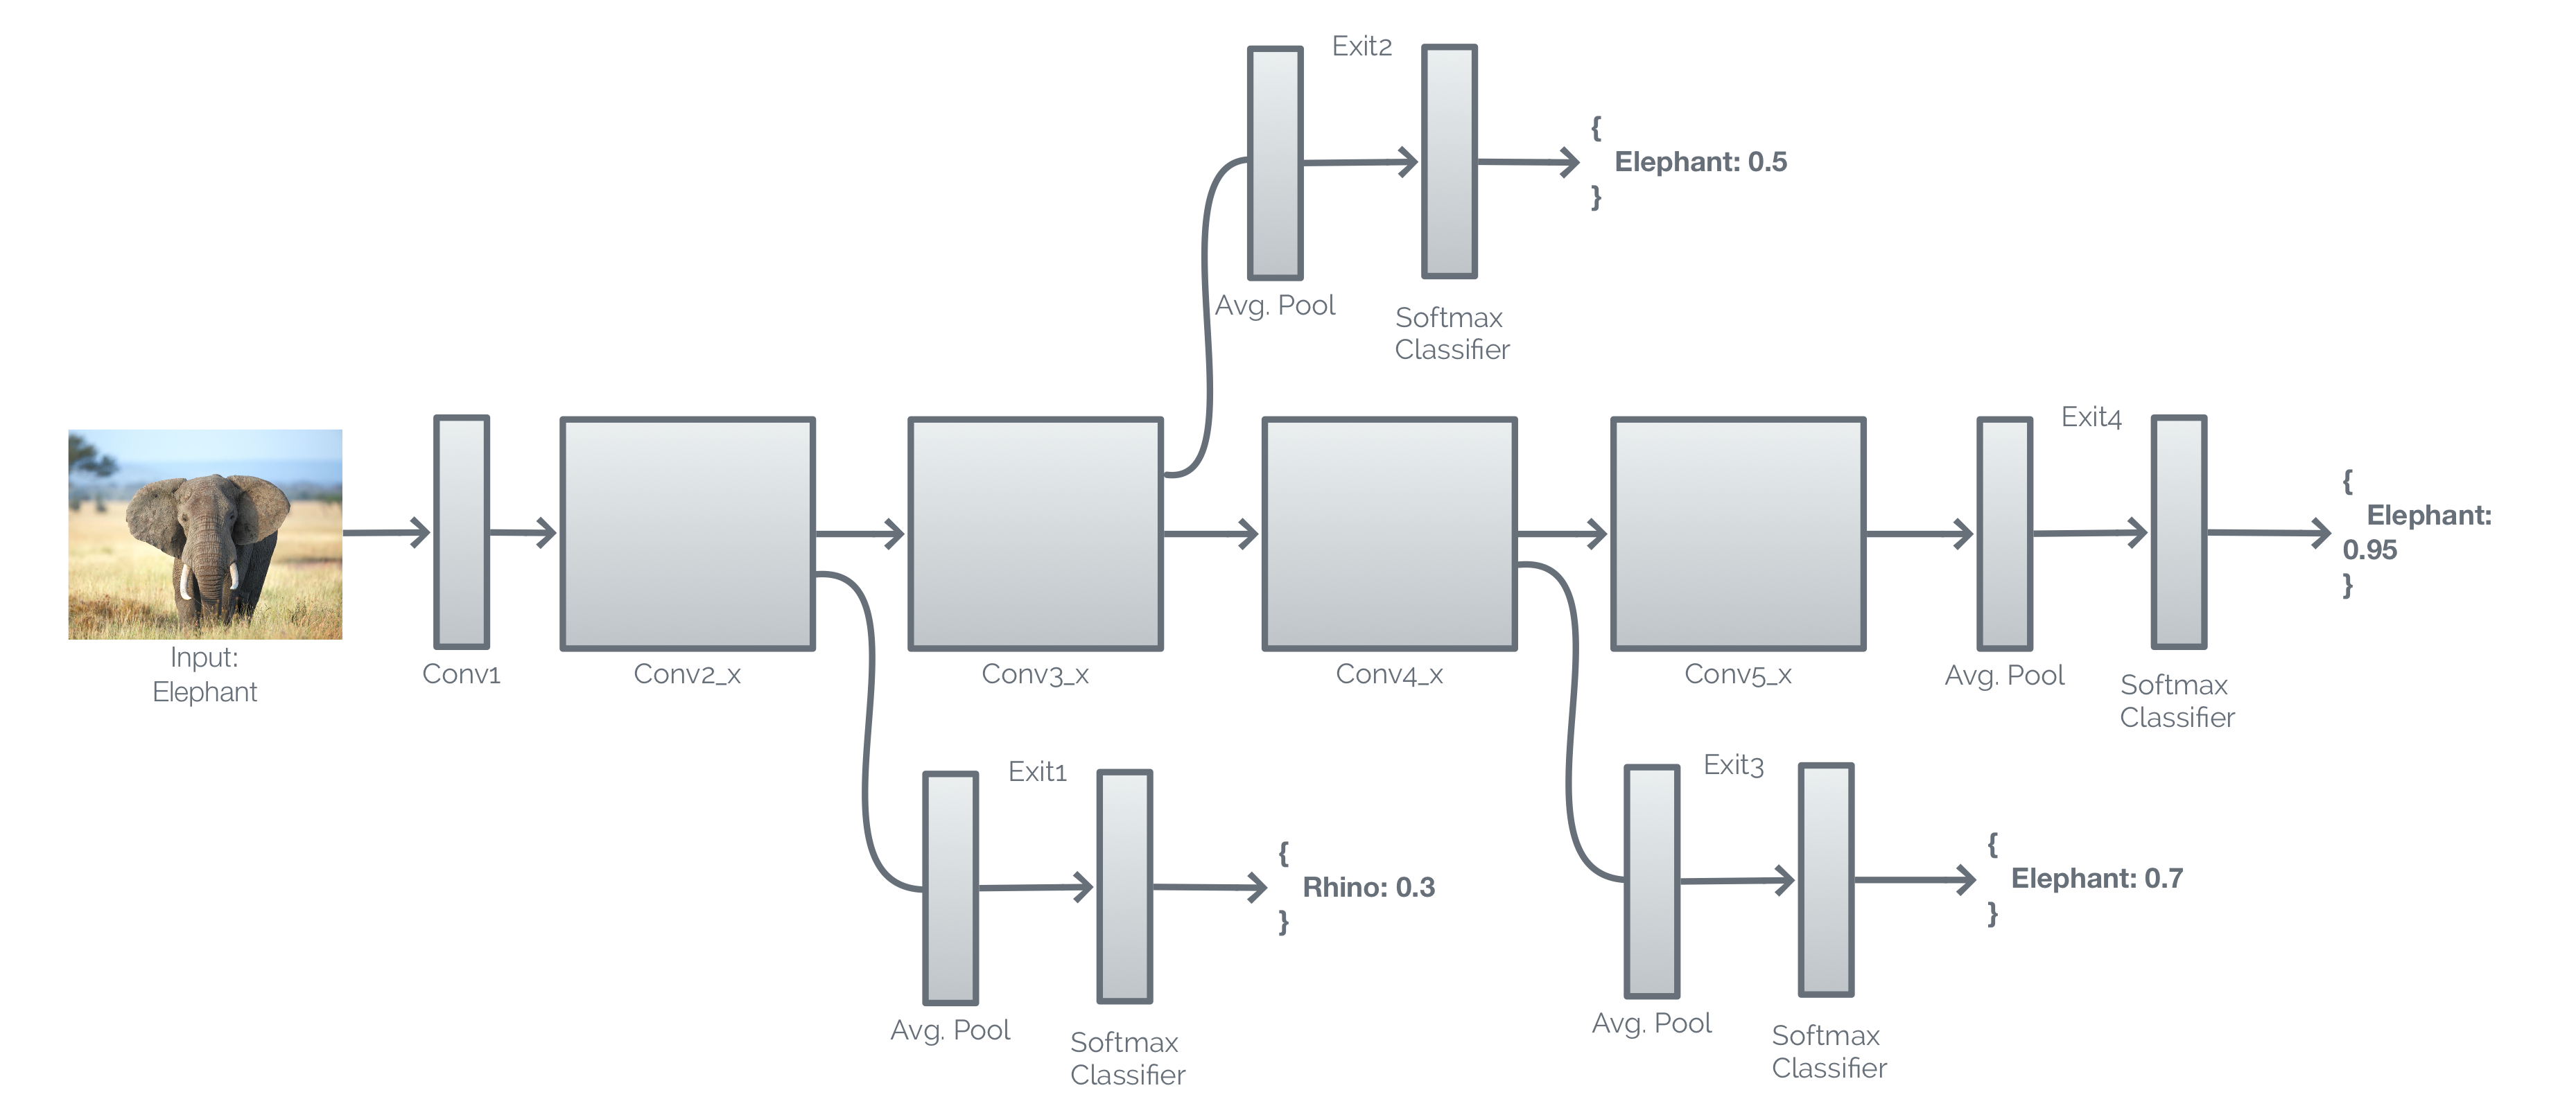
\includegraphics[width=\linewidth]{figures/models/BResNet}
	\caption[B-\gls{resnet} architecture]{Branchy-\gls{resnet}101: \gls{resnet}101 extended to implement the BranchyNet framework. The figure illustrates how classification confidence grows, as we go deeper in the model. The first exit actually fails to classify the elephant. }
	\label{fig:b-resnet}
\end{figure}


\subsection{Branchy-DenseNet}

In this section is the dense layers, the building block of the densely connected network, is explained. Followed by a design description of Branchy-\gls{densenet}.

DenseNet \cite{huang_densely_2016} is build on the assumption, that many layers of a \gls{resnet} only have a small contribution to the output and can in fact be dropped during training \cite{huang_densely_2016}. Instead of adding previously learned information to the output, \gls{densenet} combines features from all subsequent layers by concatenation, as there is no need to relearn redundant information. Figure \ref{fig:denseblock} show the dense connections, that combine features from previous layers and how the features size grows throughout a densely connected block \todo{maybe a bit sharper explanation and more figure near.}

%\begin{figure}
%	\centering
%	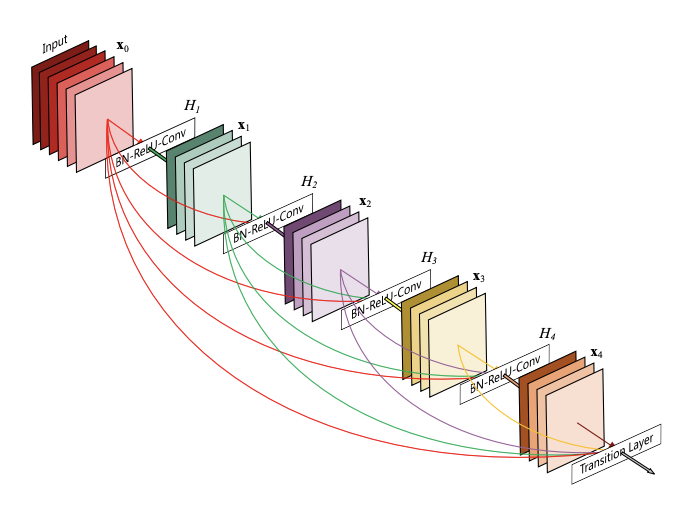
\includegraphics[width=.5\linewidth]{figures/models/denseblock}
%	\caption[Densely Connected Block]{Densely Connected Block}
%	\label{fig:denseblock}
%\end{figure}

The densely connected layers are similarly to residual network grouped into resolution block called dense blocks, but for \gls{densenet} intermediate transition layers are added between dense block to downsample the feature size. 

\begin{figure}
	\centering
	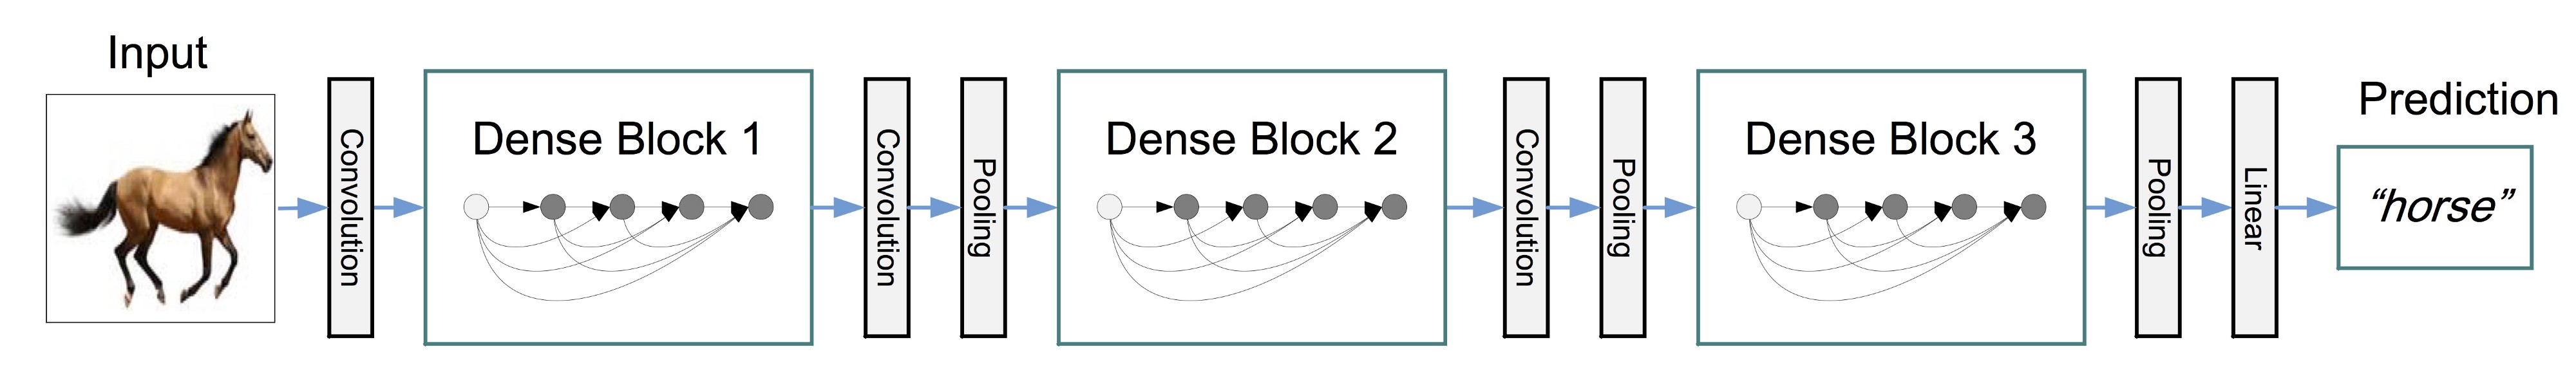
\includegraphics[width=\linewidth]{figures/models/densenet}
	\caption[Densely Connected Block]{Densely Connected Block}
	\label{fig:densenet}
\end{figure}

The collective knowledge from all preceding layers gives more diversified features compared to the correlated features of \gls{resnet}s. In \cite{huang_multi-scale_2017} the diversified features are shown to be more suited for early exiting,  as the information are better preserved using dense connection, hence even though information may have been collapsed to generate a short-term feature for the classifier. Thus placement of an intermediate classifier have less impact on the learned features for a later classifier. \gls{densenet} can be thinner as the number of channel can be fewer, thus more efficient compared to traditional and residual networks. Additionally densely connected blocks have a regularizing effect thus reducing overfitting the training data, hence perform better on smaller training sets. 

Table \ref{tbl:densenet121} describes the block and layers of the \gls{densenet} architecture. 

\begin{minipage}{\linewidth}
\begin{longtabu}{>{\bfseries}X|X[c]|X[2c]}
	\caption[\gls{densenet}-121 description]{\gls{densenet}-121 description. The table describes the blocks of \gls{densenet}-121. $k$ is the growth rate of the DenseBlock. A typical setting is $k=32$ yielding 256, 512 and 1024 output channels for denseblock(1-3) respectively. The transition layer downsamples the output channel by a factor of 2, thus the number of input channels for DenseBlock(2-4) becomes 128, 256 and 512 respectively.} \label{tbl:densenet121} \\
	\toprule
	\rowfont{\bfseries}
	Layers & Output size & Layer description \tabularnewline
	\hline
	\endfirsthead
	\multicolumn{3}{@{}l}{\textbf{\textcolor{black}{Table \ref{tbl:resnet50}:}} continued}\\
	\toprule
	\rowfont{\bfseries}
	Layers & Output size & Layer description \tabularnewline
	\hline
	\endhead % all the lines above this will be repeated on every page
	\hline
	\multicolumn{3}{@{}l}{continued \ldots}\\
	\endfoot
	\hline
	\endlastfoot
	Convolution & $112\times 112$& $7\times 7, \:\mathrm{stride}\: 2$ \tabularnewline \hline
	Pooling & $56\times 56$& $3\times 3, \:\mathrm{maxpool},\:  \mathrm{stride}\: 2$ \tabularnewline \hline
	\multirow{3}{*}{DenseBlock (1)} 	& \multirow{3}{*}{$56 \times 56$} & \multirow{3}{*}{
		$\begin{bmatrix}
		1 \times 1, k \\ 3 \times 3, k \\
		\end{bmatrix} \times 6$ }		\tabularnewline										
	& &  	\tabularnewline
	& & 	\tabularnewline
	\hline
	
	Transition  	& $56 \times 56$ & $1 \times 1\: \mathrm{conv}$ \tabularnewline \tabucline{2-3}							
	Layer (1) & $28\times 28$ & $2\times 2\: \mathrm{average\: pool,\: stride}\: 2$	\tabularnewline
	
	\hline
	
	\multirow{3}{*}{DenseBlock (2)} 	& \multirow{3}{*}{$28 \times 28$} & \multirow{3}{*}{
		$\begin{bmatrix}
		1 \times 1, k \\ 3 \times 3, k \\
		\end{bmatrix} \times 12$ }		\tabularnewline										
	& &  	\tabularnewline
	& & 	\tabularnewline
	\hline
	
	Transition  	& $28 \times 28$ & $1 \times 1\: \mathrm{conv}$ \tabularnewline \tabucline{2-3}							
	Layer (2) & $14\times 14$ & $2\times 2\: \mathrm{average\: pool,\: stride}\: 2$	\tabularnewline
	
	\hline
	
	\multirow{3}{*}{DenseBlock (3)} 	& \multirow{3}{*}{$14 \times 14$} & \multirow{3}{*}{
		$\begin{bmatrix}
		1 \times 1, k \\ 3 \times 3, k \\
		\end{bmatrix} \times 24$ }		\tabularnewline										
	& &  	\tabularnewline
	& & 	\tabularnewline
	\hline
	
	Transition  	& $14 \times 14$ & $1 \times 1\: \mathrm{conv}$ \tabularnewline \tabucline{2-3}							
	Layer (3) & $7\times 7$ & $2\times 2\: \mathrm{average\: pool,\: stride}\: 2$	\tabularnewline
	
	\hline
	
	\multirow{3}{*}{DenseBlock (4)} 	& \multirow{3}{*}{$7 \times 7$} & \multirow{3}{*}{
		$\begin{bmatrix}
		1 \times 1, k \\ 3 \times 3, k \\
		\end{bmatrix} \times 16$ }		\tabularnewline										
	& &  	\tabularnewline
	& & 	\tabularnewline
	\hline
	
	Classification  	& $1 \times 1$ & $7 \times 7\: \mathrm{global\: average\: pool}$ \tabularnewline \tabucline{2-3}							
	Layer &  \multicolumn2{c}{$\mathrm{Avg.\: Pool,\:} 1000d\: \mathrm{fc,\: Softmax}$} \tabularnewline
	\bottomrule
\end{longtabu}
\color{caption-color}{\textit{Source: \citetitle{huang_densely_2016}, by \citeauthor{huang_densely_2016} \cite{huang_densely_2016}, describes a full list of Densely Connected Networks (\gls{densenet}-121, \gls{densenet}-169, \gls{densenet}-201 and \gls{densenet}-264)}} \color{main-color}
\end{minipage}

In the same fashion as B-ResNet early exits have been placed to construct B-DenseNet. The exits are placed after a DenseBlock to obtain feature of sufficient quality and exiting as quickly as possible. If used in Edge-Device mode and the confidence was insufficient the transition layer after the DenseBlock is executed, before data is being preprocess for offloading.

\section{Experimental Setup} \label{sec:ee-exp-setup}

All code is written in \gls{python} 3.7 \cite{van_rossum_python_1995} using the \gls{pytorch} 1.2
framework \cite{paszke_automatic_2017} and using the \gls{torchvision} 0.4 library \cite{marcel_torchvision_2010}. All code is available at:
{\color{sns-grey}\url{https://github.com/AlexKarlsen/thesis-src}}. 

Table \ref{tbl:platforms} lists the hardware and its characteristics used for the experiments. Table \ref{tbl:models} lists the models used in the experiment and compares the number of layers, parameters and \gls{flop}s of the models. The number of parameters and \gls{flop}s have been found using \gls{thop} \cite{zhu_thop_nodate}, by inference a random 4d tensor of size $ (\mathrm{batch,channels,width,height})=(1,3,224,224) $ to all models.
 
\begin{longtabu}{>{\bfseries}X[0.8]|X[0.8]|X[1.5]|X[r0.3]}
	\caption[Platform hardware comparison]{Platform hardware comparison of Window 10 Stationary PC and NVIDIA Jetson TX2 Edge Computer} \label{tbl:platforms} \\
	\toprule
	\rowfont{\bfseries}
	Platform & CPU & GPU & RAM  \tabularnewline
	\bottomrule
	\endfirsthead
	\multicolumn{3}{@{}l}{\textbf{\textcolor{black}{Table \ref{tbl:platforms}:}} continued}\\
	\toprule
	\rowfont{\bfseries}
	Platform & CPU & GPU & RAM  \tabularnewline
	\bottomrule
	\endhead % all the lines above this will be repeated on every page
	\bottomrule
	\multicolumn{3}{@{}l}{continued \ldots}\\
	\endfoot
	\hline
	\endlastfoot
	GPU Workstation	& Intel i5-6600K.	& NVIDIA GeForce GTX 1080, 2560 CUDA cores	& 16GB \tabularnewline
	\hline
	Jetson TX2	& ARM Cortex-A57 	& NVIDIA Pascal GPU, 256 CUDA cores 		& 8GB \tabularnewline
	\hline
	NUC		  	& Intel i7-7567U	& None										& 16GB \tabularnewline									
	\bottomrule
\end{longtabu}%equipped with a NVIDIA GeForce 1080 GTX \gls{gpu} using CUDA 10.1 and cuDNN 7.6.3.
\begin{longtabu}{>{\bfseries}X|X[r]|X[r]|X[r]}
	\caption[Model comparison]{ Model Parametric Comparison. The B-\gls{densenet} and \gls{msdnet} drastically reduces the mount of parameters and G\gls{flop}s compared to B-\gls{resnet}. The early exit models should be able to reduce inference delay, as they need less parameters and \gls{flop}s.}\label{tbl:models} \\
	\toprule
	\rowfont{\bfseries}
	Model  & Layers & Parameters (M) & G\gls{flop}s \tabularnewline
	\hline
	\endfirsthead
	\multicolumn{3}{@{}l}{\textbf{\textcolor{black}{Table \ref{tbl:models}:}} continued}\\
	\toprule
	\rowfont{\bfseries}
	Model & Layers & Parameters (M) & G\gls{flop}s \tabularnewline
	\hline
	\endhead % all the lines above this will be repeated on every page
	\hline
	\multicolumn{3}{@{}l}{continued \ldots}\\
	\endfoot
	\hline
	\endlastfoot
	ResNet & $ 101 $ & $ 42.705 $ & $ 7.864 $ \tabularnewline
	\hline
	DenseNet & $ 121 $ & $ 7.056 $ & $ 2.897 $ \tabularnewline
	\hline
	B-ResNet & $ 104 $ & $ 42.885 $ & $ 7.866 $ \tabularnewline 
	\hspace{3mm} Exit-0  & 11 &   0.251 & 0.807 \tabularnewline
	\hspace{3mm} Exit-1  & 13 &   1.270 & 1.041 \tabularnewline
	\hspace{3mm} Exit-2  & 70 &  26.193 & 5.206 \tabularnewline
	\hspace{3mm} Exit-3  & 11 &  15.170 & 0.812 \tabularnewline
	\hline
	B-DenseNet & $ 124 $ & $ 7.236 $ & $ 2.898 $\tabularnewline
	\hspace{3mm} Exit-0  & 14 & 0.370 & 1.183  \tabularnewline
	\hspace{3mm} Exit-1  & 26 & 1.004 & 0.836  \tabularnewline
	\hspace{3mm} Exit-2  & 50 & 3.072 & 0.668  \tabularnewline
	\hspace{3mm} Exit-3  & 34 & 2.789 & 0.211  \tabularnewline
	\hline
	MSDNet & $ 25 $ & $ 23.958 $ & $ 1.374 $ \tabularnewline
	\hspace{3mm} Exit-0  & 5 & 4.239 & 0.345 \tabularnewline
	\hspace{3mm} Exit-1  & 5 & 4.534 & 0.349 \tabularnewline
	\hspace{3mm} Exit-2  & 5 & 4.301 & 0.325 \tabularnewline
	\hspace{3mm} Exit-3  & 5 & 3.675 & 0.248 \tabularnewline
	\hspace{3mm} Exit-4  & 5 & 7.210 & 0.107 \tabularnewline
	\bottomrule
\end{longtabu}


\begin{enumdescript}
	\item[Training] All training of the models of table \ref{tbl:models} have been accomplished using the \gls{gpu}-workstation of table \ref{tbl:platforms}. In each epoch the training- and validation-, -loss and -accuracy have been logged and used for analysis in section \ref{sec:ee-results}. The trained models are available at: {\color{sns-grey}\url{https://drive.google.com/open?id=1EAl9qGxcm2U3kPhEsHp0HotgNn_LMWa1}}.
	The listed and described training hyperparameters have been used for all training sessions. 
	
	\begin{enumdescript}
		\item[Epochs] An epoch is a step of training in which every training sample have been presented to the model. A training time of 50 epochs have been selected to limit overall training time to give time for multiple attempts and training multiple model.
		
		Training the models on the available hardware took $\sim$30 to  $\sim$40 hours depending on the model. In total 5 models have been fully trained once the rest of training settings had been found.
		
		\item[Early Stopping] Early stopping is finding the best obtained model by alternating between training and validation phases for each epoch. The best model is the one obtaining the highest accuracy on the validation data. Early stopping is a mechanism to avoid overtraining a model, that then overfits the training data and obtain poor validation accuracy. For \gls{branchynet} we use the model with the highest average accuracy to not favor any part of the model.  
		
		\item[Exit Weights] The same unit weights have been selected for all exits of the model again not to favor any part of the model. In \cite{teerapittayanon_branchynet:_2016} they claim, that putting more weight on early branches have a regularizing impact on the later classifiers and can actually achieve better performance. However, they too have chosen the same unit weights for all branches, for comparison of multiple models and avoid time consuming search for specific branch weights on a per model basis.
		
		\item[Optimizer] The weights of \gls{dnn}s are typically trained using a variant of \gls{sgd} \cite{goodfellow_deep_2016}. \gls{sgdr} \cite{loshchilov_sgdr:_2016} have shown faster convergence on a number of datasets, due to its ability to escape local minimas. It follows a cyclic learning rate schedule in contrast to former decaying learning rate schedules. It has shown, in general, to perform better than adaptive optimizers such as Adam \cite{kingma_adam:_2014}, which implement adaptive learnining rate to avoid being stuck in local minimas. 
		
		\gls{sgdr} uses an aggressive cosine annealing schedule with warm restarts. Figure \ref{fig:cosineannealing} illustrates the learning rate schedule.
		
		\begin{minipage}[t]{\linewidth}
			\centering
			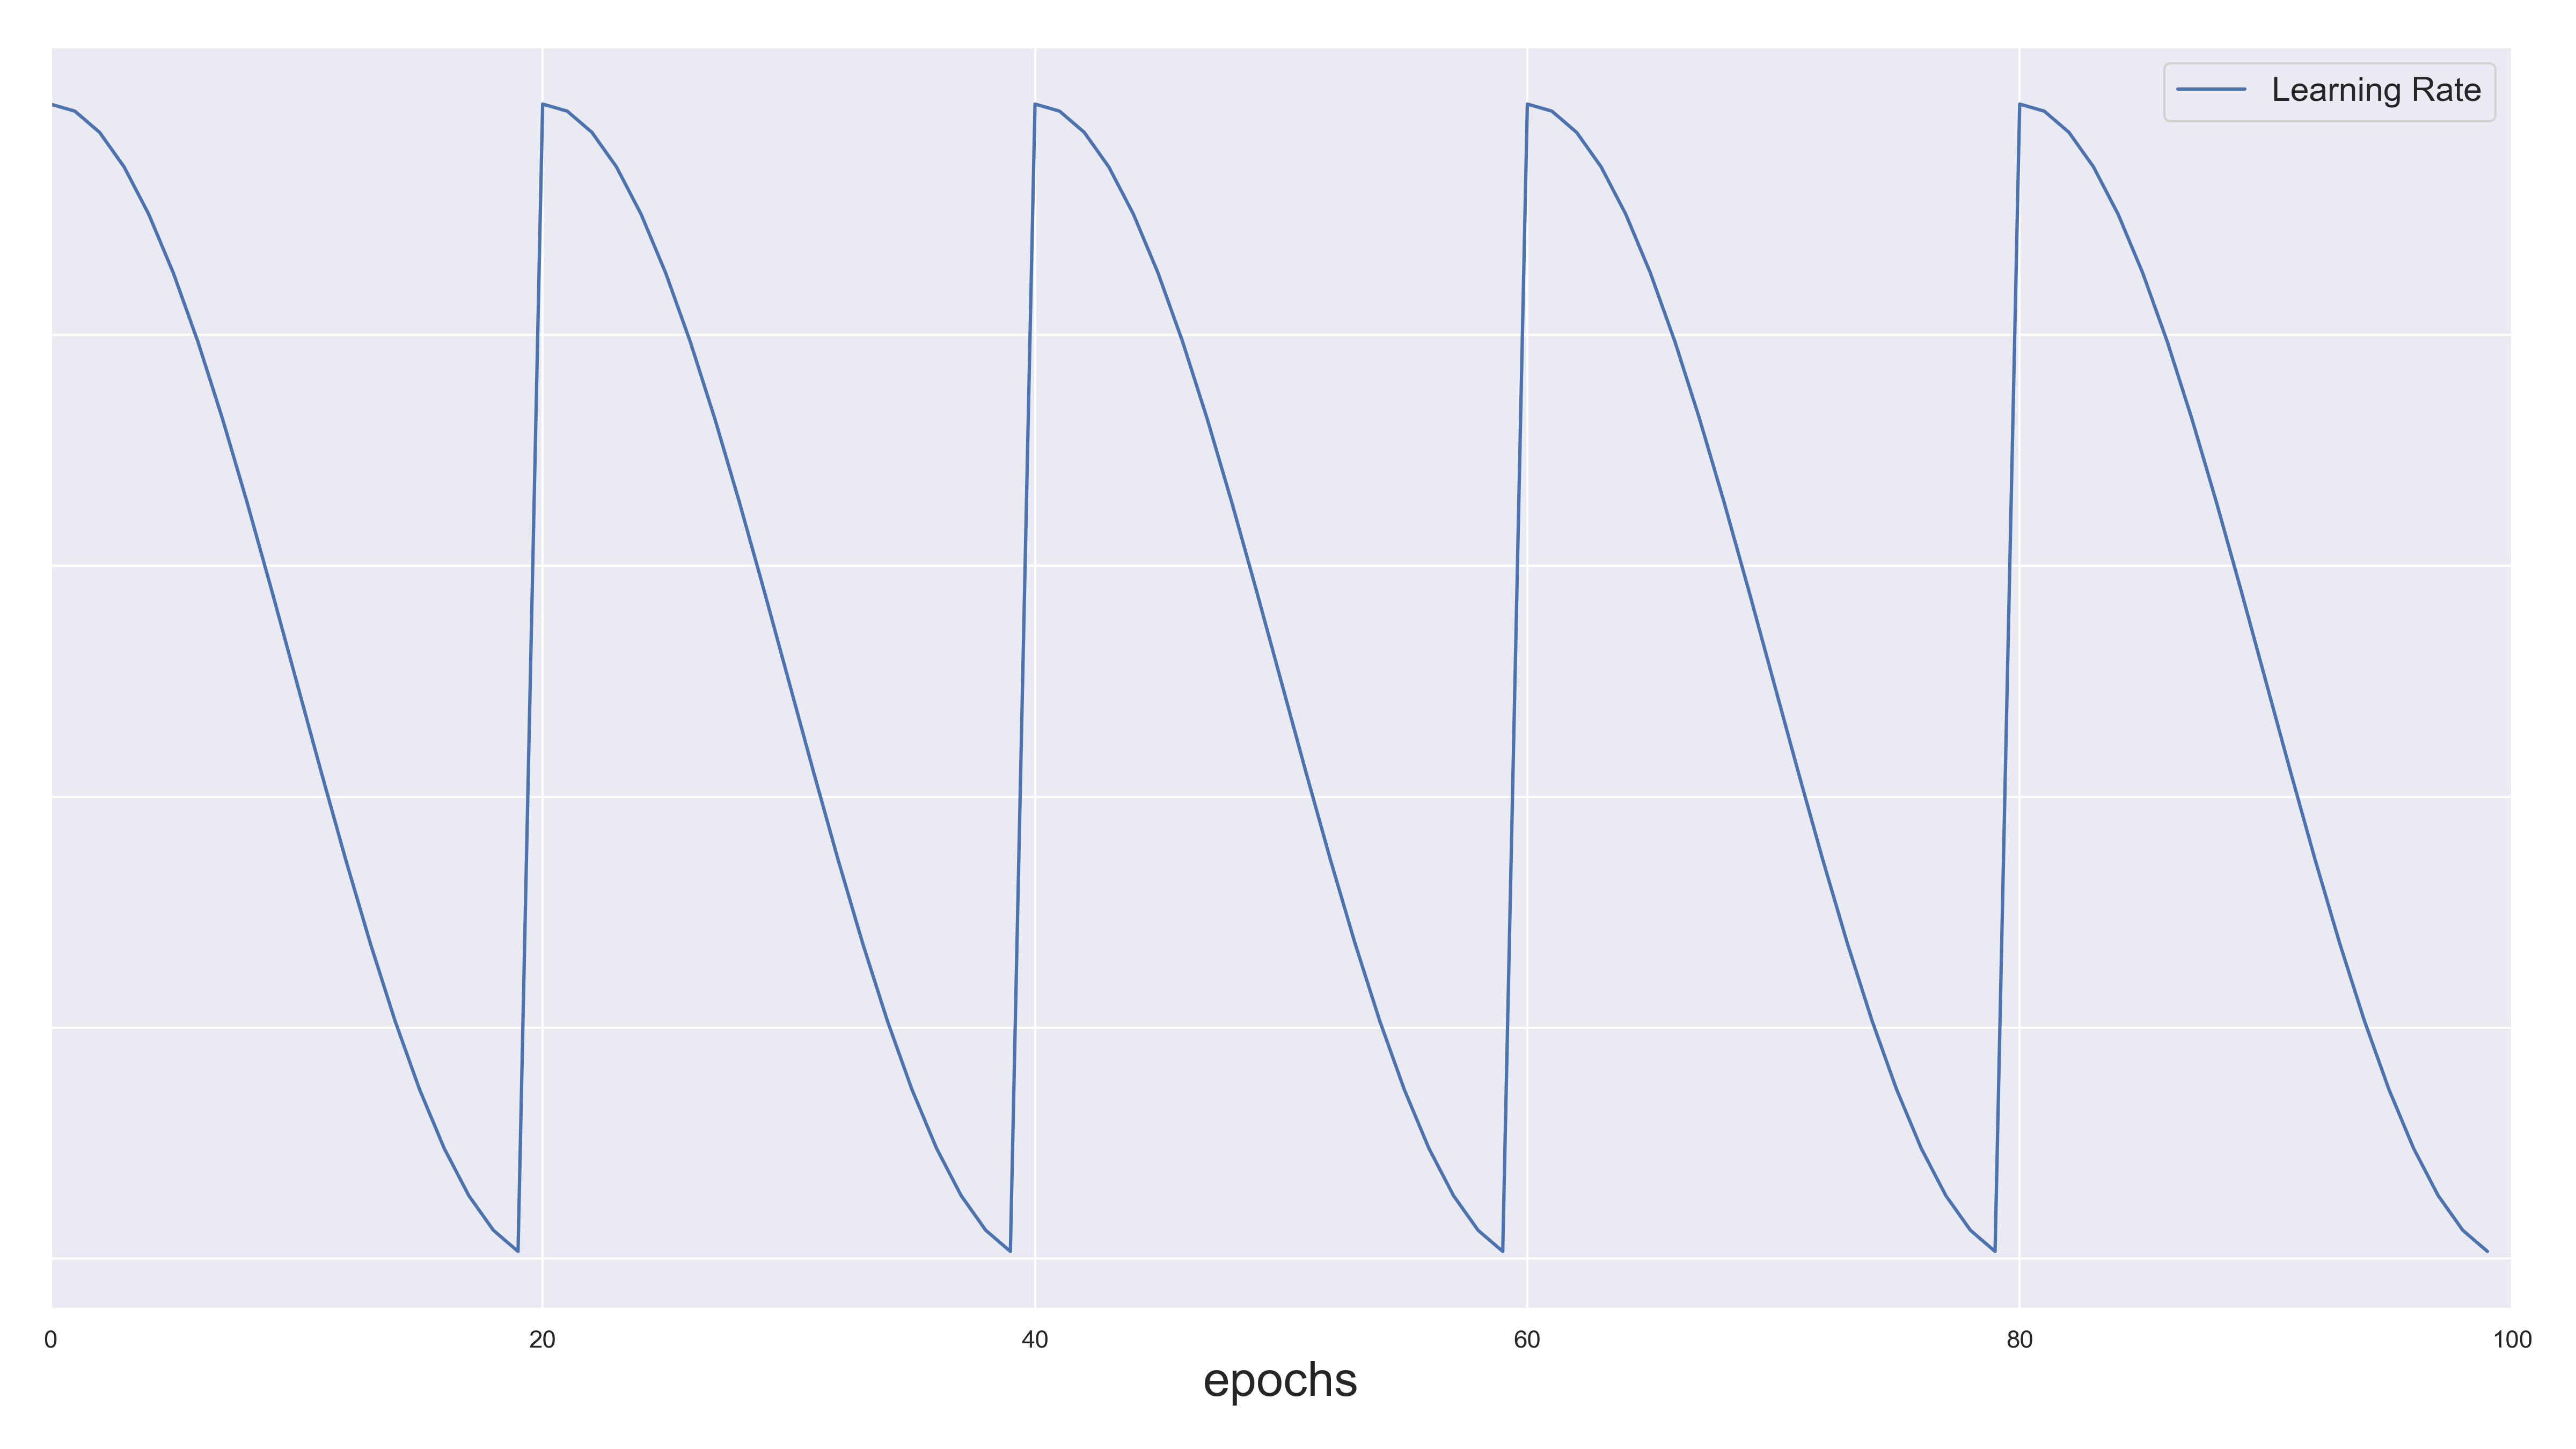
\includegraphics[width=.7\linewidth]{figures/lr.png}
			\captionof{figure}[Cosine Annealing Learning Rate]{Cosine Annealing Learning Rate} 
			\label{fig:cosineannealing}
		\end{minipage}
		
		\item[Batch Size] Batch Size are recommend to be between 1 and a few hundreds \cite{bengio_practical_2012}. To better utilize \gls{gpu}s a batch size in the power of 2 gives better runtime, e.g. 32 to 256 \cite{goodfellow_deep_2016}. Larger batch sizes have been driving by advancements in parallelism \cite{dean_large_2012}, which can improve the training time, however smaller batch size, have shown better generalization performance due to a regularizing effect \cite{masters_revisiting_nodate}, which especially large model, that tends to overfit can benefit from \cite{goodfellow_deep_2016}. 
		
		A batch size of 16 was found to be the maximum power of 2 possible with the computational budget of 8Gb RAM. The standard choice of 32 caused memory exhaustion. However, a batch size of 16 provide decent training times and may provide additional regularization over 32. Smaller batch sizes were not experimented with due to time constraints. The batch size of 16 was chosen for all \gls{dnn} training sessions.
		
		\item[Datasets] \gls{min100} is a subset of the \gls{ilsvrc2012} dataset \cite{russakovsky_imagenet_2015} created for this project, to reduce training time from several weeks to only days on available hardware. The subset is inspired by MiniImageNet \cite{vinyals_matching_2016}, that uses a subset of 100 classes with 600 samples for each class. \gls{min100} contains 100 out of 1.000 randomly sampled classes, which gives 127.300 out of 1.2m training samples and 5.000 out of 50.000 validation samples. A full list of classes are found in the table \ref{tbl:min100}. 
		
		Compared to other sufficiently dense classification datasets e.g \gls{tinyimagenet} \cite{li_cs231n:_2018}, \gls{cifar10} and \gls{cifar100} \cite{krizhevsky_cifar-10_nodate}, the image sizes of these datasets are respectively $(64\times 64$), $(32\times 32)$, $(32\times 32)$ pixels, all of which are considered too small for this project. Other datasets such as MS COCO and Pascal VOC are better suited for object detection/segmentation, as images are not cropped to only focus on a single object, thus too challenging for classification. In fact Pascal VOC was initially tested, the model however, clearly overfitted the training data due to data sparsity. 
		
		\item[Image Augmentation] A models ability generalize a specific classification problem has a close connection with the number of available training samples. Data augmentation haven proven to be powerful tool in order to virtually create more training data \cite{perez_effectiveness_2017}. Enlarging a training dataset by data augmentation can help create new versions of an image, that are different from but still similar to the original image, without actually having to acquire and annotate new samples \cite{goodfellow_deep_2016}.  
		
		\begin{minipage}[t]{\linewidth}
			\centering
			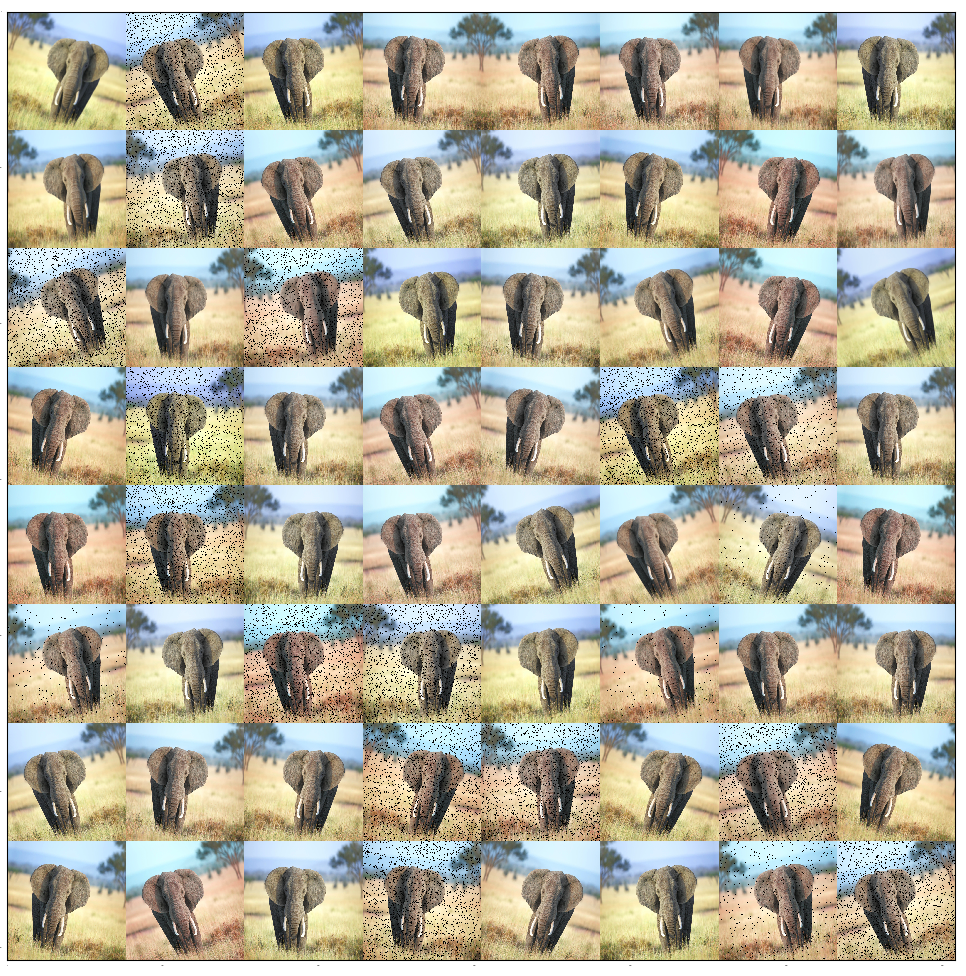
\includegraphics[width=.7\linewidth]{figures/augmentation/augmentation_high_resolution.png}
			\captionof{figure}[Image Augmentaion Example]{Image Augmentation of an elephant}
			\label{fig:augmentation}
		\end{minipage}
		
		Image augmentation involves transformations using tools from image processing to randomly apply noise injection, and color space transformations including contrast and saturation distortions, as well as geometric transformations, such as simple transformations of flipping the image to more complex affine transformations to create different image perspectives \cite{shorten_survey_2019}. Figure \ref{fig:augmentation} shows 64 random augmentations of an image of an elephant, achieved using \gls{imgaug} \cite{jung_imgaug:_nodate}. 
		
		New methods have been proposed where image transformations are learned to improve generalization e.g. AutoAugment \cite{cubuk_autoaugment:_2018}. 
		
		Other methods involves actually enlarging the training dataset by synthetically creating more data using a \gls{gan}. \gls{gan}s can help overcome limited data given the available training data or a 3D model, by artificially constructing synthetic samples in different background, light setting and from alternate perspectives.
		
		Methods that do not cover enriching the available training, but alters the learning procedure are called regularization and covers; weight decay, dropout, batch normalization etc. We do not experiment with these regularization technique, but uses the settings set in the implementation of the models.
		
		\item[Transfer Learning] Transfer learning is the procedure of using a pre-trained model to train on a new dataset, under the assumption, that features learned on one image dataset can be reused for another dataset \cite{yosinski_how_2014}. Typically models have been pre-trained on the ImageNet dataset. The density of the dataset enables models to learn general features suitable for other domains \cite{kornblith_better_2019}. Transfer learning are especially suited for when the new data domain is of limited quantity and the similarities between the two data domains are strong. If the similarity is weak a model can be partially trained, the shallow layers containing general features are frozen and only the deeper layers with more specialized features are fine-tuned for the new data domain \cite{li_cs231n:_2018}. Thus, transfer learning can reduce the training time to learn general features of shallow layers and possibly learn more specific features at deeper layers, adapted to the new dataset.
	\end{enumdescript}
	
	\item[Inference] The inference experiment have been conducted by letting all samples inference the model, the output and measured time of all exits have been logged and used for analysis in section \ref{sec:ee-results}. All hardware of table \ref{tbl:platforms} and all trained models of table \ref{tbl:models} have been used. The inference experiment does not require nearly the same amount of setting as the training does, those required are listed here:
	\begin{enumdescript}
		\item[Batch Size] A batch size of 1 have been chosen to simulate a real scenario, and to measure time of each samples
		\item[Dataset] The validation dataset of \gls{min100} containing 5000 samples have been used.
	\end{enumdescript} 
	
\end{enumdescript}

\section{Results} \label{sec:ee-results}

\subsection{Training Results}

We trained the three early exiting models B-\gls{resnet}, B-\gls{densenet} and \gls{msdnet}, along with conventional versions of the \gls{resnet}101 and \gls{densenet}-121. The \gls{dnn}s were trained on the \gls{min100} training set..

First we trained B-\gls{resnet} using transfer learning from the ImageNet dataset. We froze the features of the network and only trained the classifiers of all the exits. Figure \ref{fig:frozen-b-resnet-miniimagenet-100} show the results from the training. The figure shows, that the features learned from a conventional single exit model, are not suitable for an early exit model. None of the intermediate classifiers are able to obtain acceptable accuracy on neither the training nor the validation set. The features for the shallower part of the network are not optimized for the early classifiers. This study clearly reveals the need to train the entire model, to obtain an early exit model with decent accuracy.  

\begin{figure}
	\centering
	\captionsetup[subfigure]{justification=centering, farskip=1pt,captionskip=1pt}
	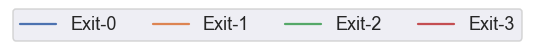
\includegraphics[width=.5\textwidth]{figures/training_plots/frozen_b-resnet_exit_legend}
	\subfloat[Train loss\label{fig:frozen-b-resnet-train-loss}]{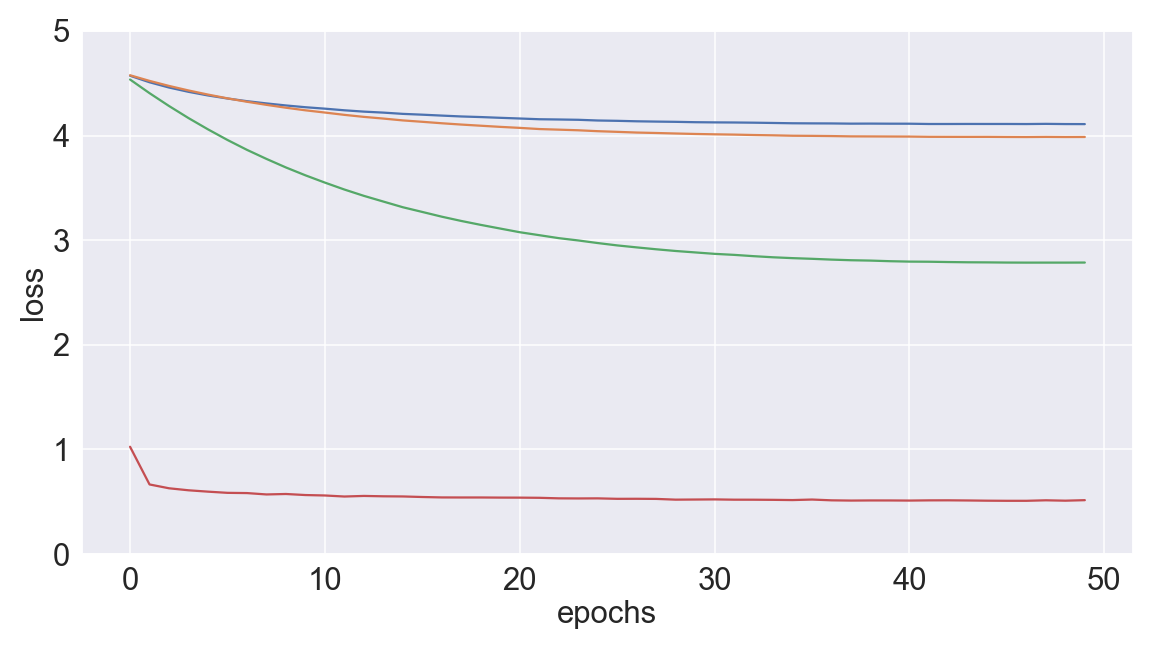
\includegraphics[width=.49\textwidth]{figures/training_plots/frozen_b-resnet_train-loss}}
	\subfloat[Test loss \label{fig:frozen-b-resnet-test-loss}]{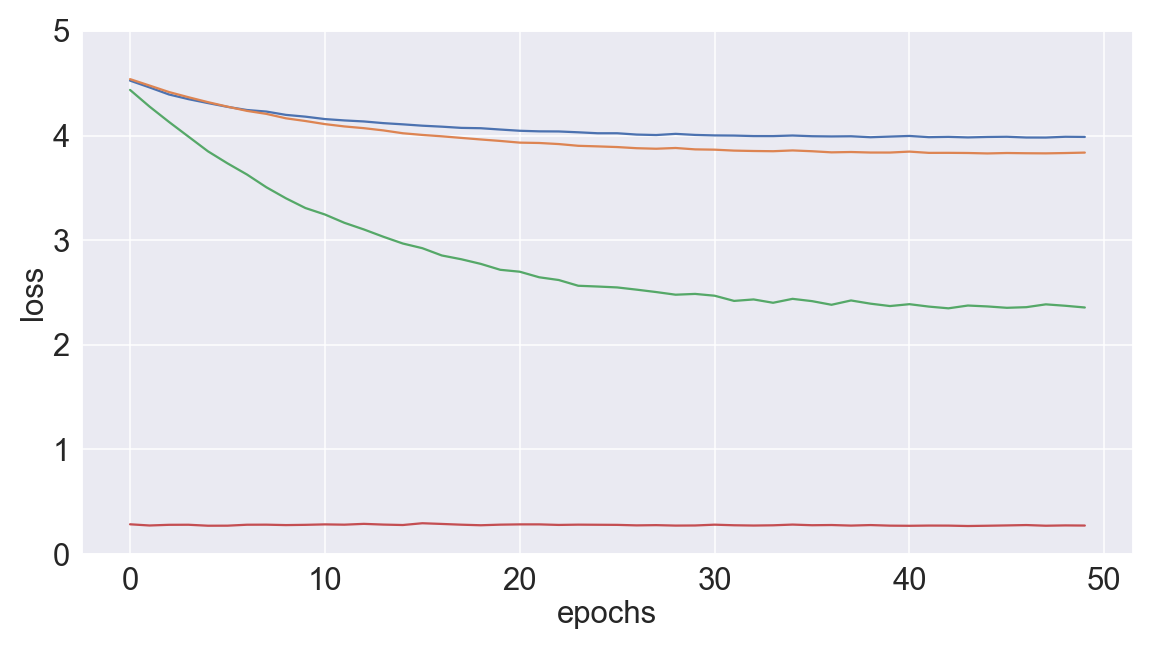
\includegraphics[width=.49\textwidth]{figures/training_plots/frozen_b-resnet_test-loss}}
	\hfill
	\subfloat[Train accuracy\label{fig:frozen-b-resnet-train-acc}]{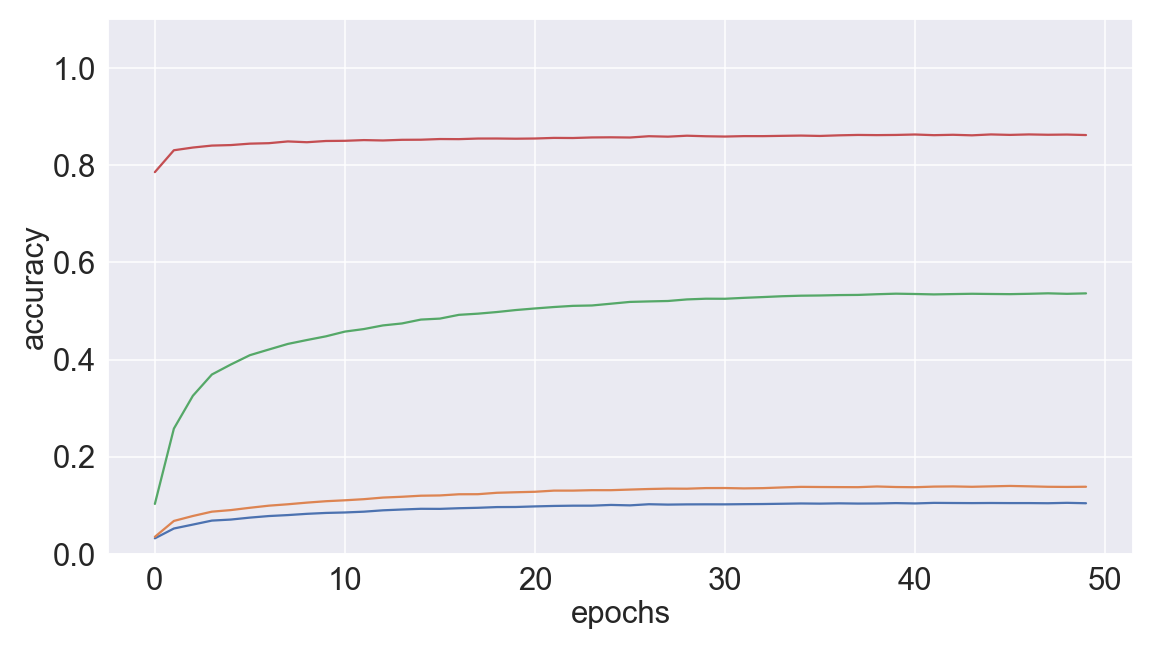
\includegraphics[width=.49\textwidth]{figures/training_plots/frozen_b-resnet_train-accuracy}}
	\subfloat[Test accuracy\label{fig:frozen-b-resnet-test-acc}]{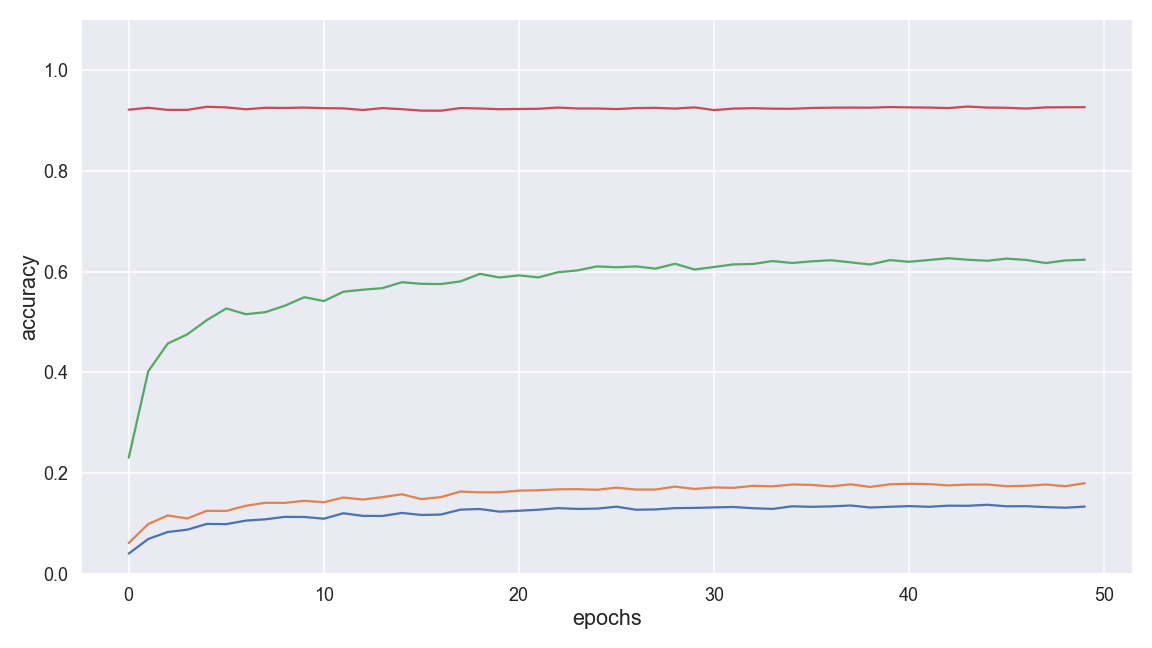
\includegraphics[width=.49\textwidth]{figures/training_plots/frozen_b-resnet_test-accuracy}}
	\caption[Frozen Bresnet Training summary]{Frozen B-resnet Training summary: shows the progression of model attributes over times of epochs, \protect\subref{fig:frozen-b-resnet-train-loss} train loss, \protect\subref{fig:frozen-b-resnet-test-loss} test loss, \protect\subref{fig:frozen-b-resnet-train-acc} train accuracy, \protect\subref{fig:frozen-b-resnet-test-acc}, test accuracy.}
	\label{fig:frozen-b-resnet-miniimagenet-100}
\end{figure}

As found in \cite{teerapittayanon_branchynet:_2016}, we unfreeze the model, to allow the features of the model to be optimized for the intermediate classifiers of the early exit model. Figure \ref{fig:b-resnet-miniimagenet-100} show the training results. The accuracy at early exits classifiers are greatly improved by 140 \% to almost 390 \%. However, the accuracy of the final classifier are reduced by 4 \%. The reduction in accuracy may be caused by;
\begin{enumerate}
	\item The features of the third and largest resolution block just before exit-2, see table \ref{tbl:resnet101}, may be optimized too much for exit-2, thus collapses the information, that the last block should use to learn more descriptive features. 
	\item It could be a sign of overfitting, due to the size of dataset is only $\frac{1}{10}$ of the dataset used to train the original model. 
\end{enumerate}
However, the last two exits obtain a training accuracy close to 1. However, there is no notable degradation in validation loss or accuracy, which would have been the clearest sign of overfitting. We did also train conventional versions of the two models on the same datasets, and since both models are able to obtain over 0.9 in accuracy, we argue, that the most probable reason is optimization to earlier exit, as the same trend is shown in \cite{huang_multi-scale_2017}.

\begin{figure}
	\centering
	\captionsetup[subfigure]{justification=centering, farskip=1pt,captionskip=1pt}
	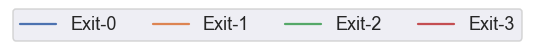
\includegraphics[width=.5\textwidth]{figures/training_plots/b-resnet_exit_legend}
	\subfloat[Train loss\label{fig:b-resnet-train-loss}]{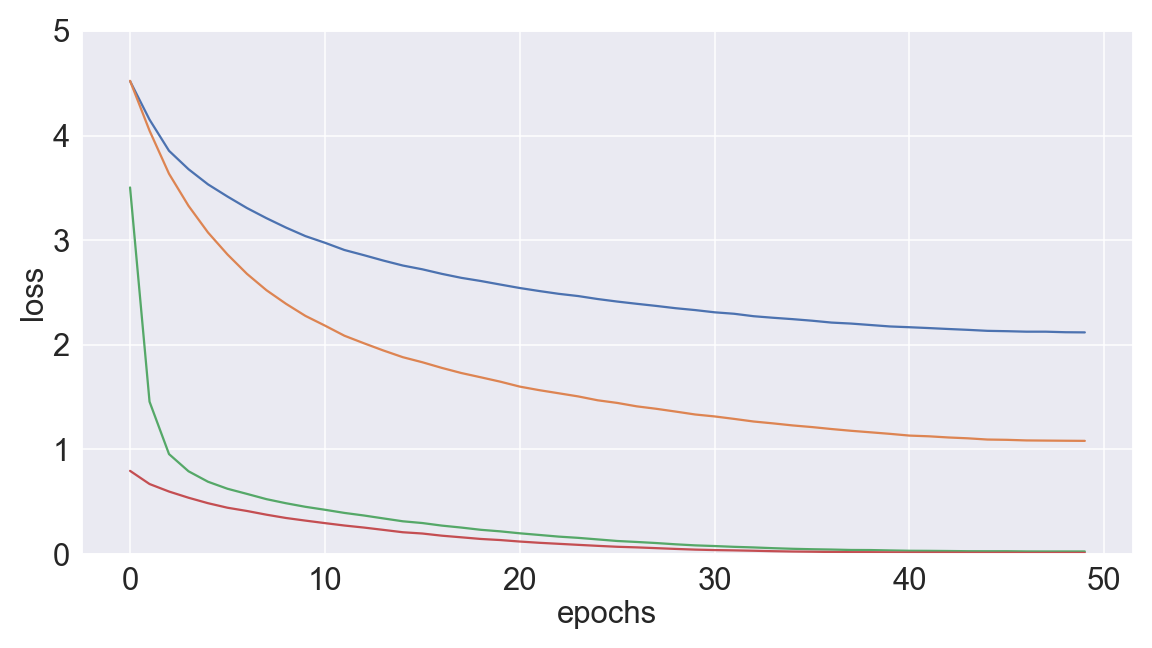
\includegraphics[width=.49\textwidth]{figures/training_plots/b-resnet_train-loss}}
	\subfloat[Test loss \label{fig:b-resnet-test-loss}]{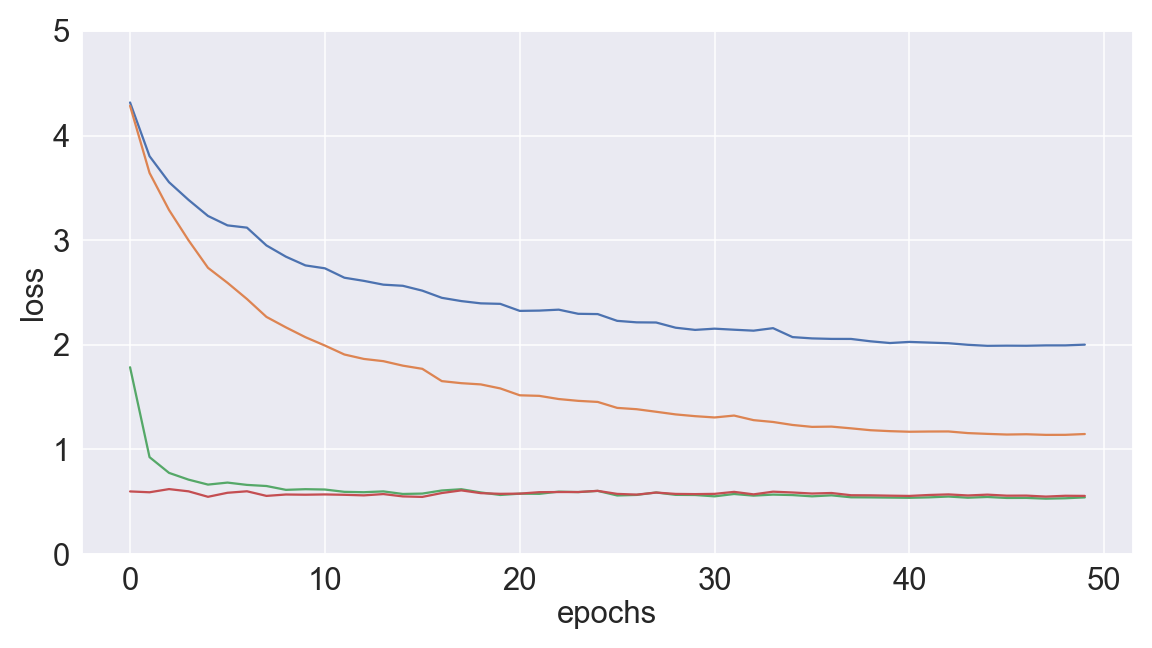
\includegraphics[width=.49\textwidth]{figures/training_plots/b-resnet_test-loss}}
	\hfill
	\subfloat[Train accuracy\label{fig:b-resnet-train-acc}]{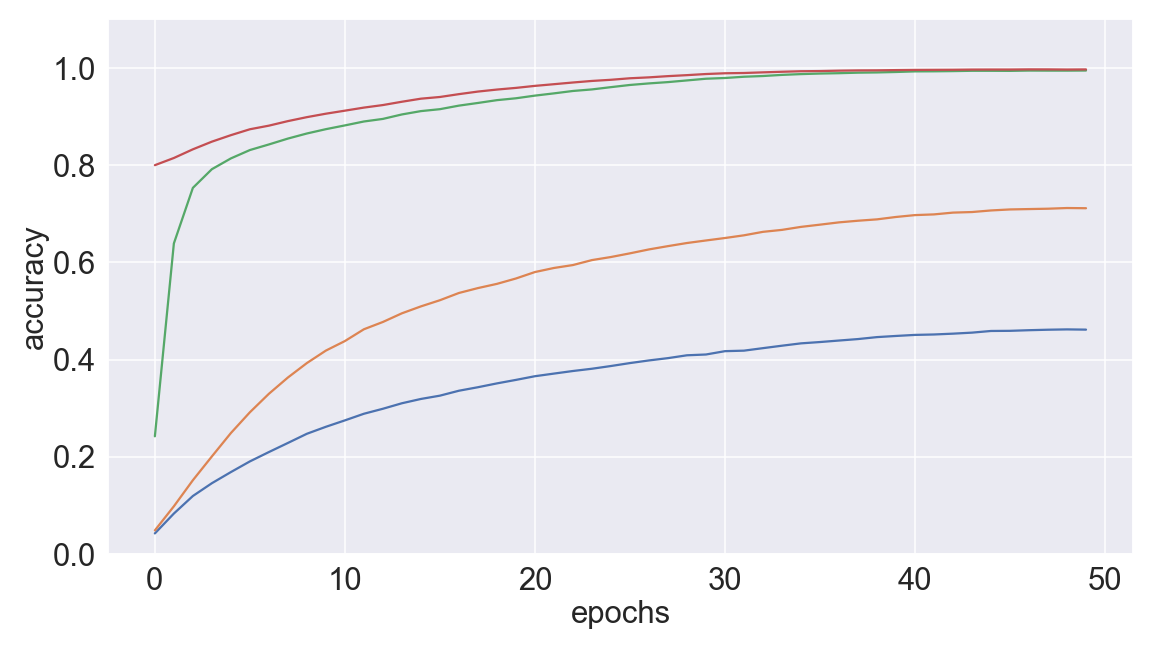
\includegraphics[width=.49\textwidth]{figures/training_plots/b-resnet_train-accuracy}}
	\subfloat[Test accuracy\label{fig:b-resnet-test-acc}]{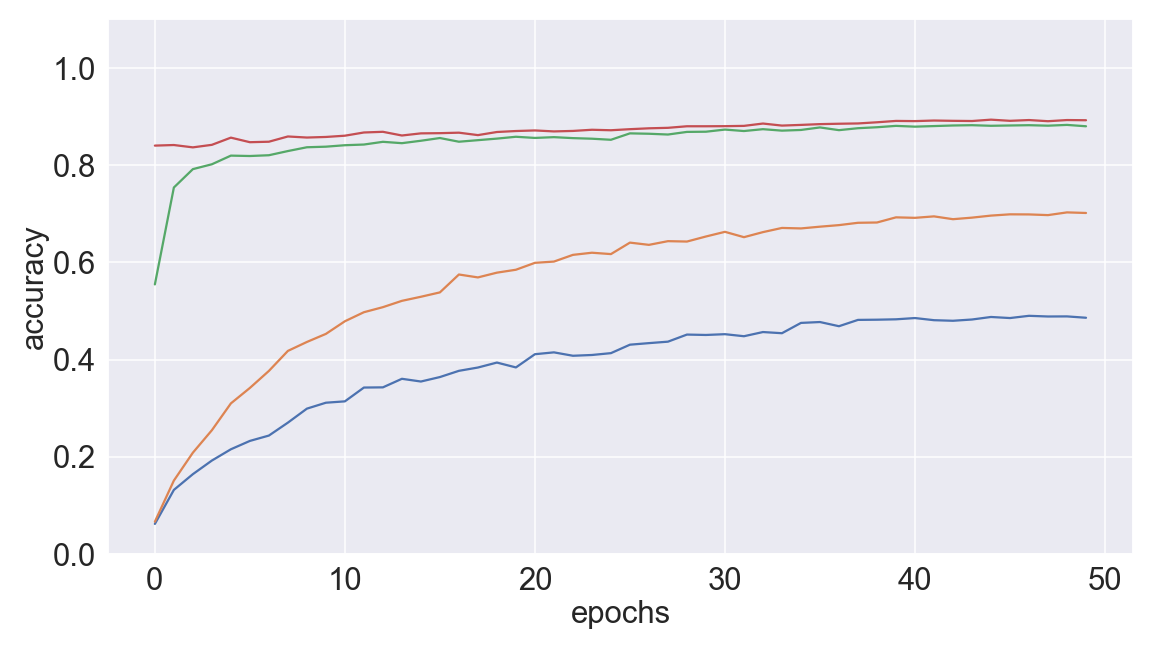
\includegraphics[width=.49\textwidth]{figures/training_plots/b-resnet_test-accuracy}}
	\caption[B-ResNet Training summary]{B-ResNet Training summary: shows the progression of model attributes over times of epochs, \protect\subref{fig:b-resnet-train-loss} train loss, \protect\subref{fig:b-resnet-test-loss} test loss, \protect\subref{fig:b-resnet-train-acc} train accuracy, \protect\subref{fig:b-resnet-test-acc}, test accuracy.}
	\label{fig:b-resnet-miniimagenet-100}
\end{figure}

Table \ref{tbl:frozen-vs-unfrozen}  shows the improvement of the higest validation score obtained in the training process. Comparing the two show, that we are able to improve the accuracy at early exits, thus the features located in the shallower part of the model now provides information that enables the classifiers to better discriminate the classes. 

\begin{longtabu}{>{\bfseries}X[2]|X|X|X|X}
	\caption[Comparison of Transfer Learning Approaches]{Comparison of transfer learning approaches frozen model vs. fine-tuning on validation accuracy} \label{tbl:frozen-vs-unfrozen} \\
	\toprule
	\rowfont{\bfseries}
	Model & Exit-0 & Exit-1 & Exit-2 & Exit-3 \tabularnewline
	\bottomrule
	\endfirsthead
	\multicolumn{3}{@{}l}{\textbf{\textcolor{black}{Table \ref{tbl:frozen-vs-unfrozen}:}} continued}\\
	\toprule
	\rowfont{\bfseries}
	Model & Exit-0 & Exit-1 & Exit-2 & Exit-1 \tabularnewline
	\bottomrule
	\endhead % all the lines above this will be repeated on every page
	\bottomrule
	\multicolumn{3}{@{}l}{continued \ldots}\\
	\endfoot
	\hline
	\endlastfoot
	Frozen B-\gls{resnet}	& 0.14	& 0.18	& 0.63 & 0.93 \tabularnewline
	\hline
	Unfrozen B-\gls{resnet}	& 0.49 	& 0.70 & 0.88 & 0.89 \tabularnewline
	\hline
	Change & 350 \% & 389 \% & 140 \% &  96 \% \tabularnewline							
	\bottomrule
\end{longtabu}

As the two last exits of \gls{resnet} is almost equally accurate, not much gain is obtained by running the model all the way to the end. Figure \ref{fig:b-densenet-miniimagenet-100} show the training result of B-\gls{densenet}. B-\gls{densenet} on the other hand always have a gain in accuracy by continuing the inference process all the way to the end, and are also able to achieve better accuracy at earlier exits than B-\gls{resnet}. However, again at the cost of less accurate end exit. The figure shows the same importance of the densely connected layers for an early exit model as in \cite{huang_multi-scale_2017}. Eventhough the two first exits of B-\gls{densenet} have a higher accuracy, the last two exits obtain higher accuracy for the Figure \ref{fig:b-densenet-miniimagenet-100} show the training result of B-\gls{densenet}, see table \ref{tbl:training-compariosn}. \gls{msdnet}, the early exiting version of \gls{densenet}, shows further improvement to early exits accuracy.     

\begin{figure}
	\centering
	\captionsetup[subfigure]{justification=centering, farskip=1pt,captionskip=1pt}
	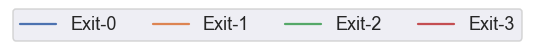
\includegraphics[width=.5\textwidth]{figures/training_plots/b-densenet_exit_legend}
	\subfloat[Train loss\label{fig:b-densenet-train-loss}]{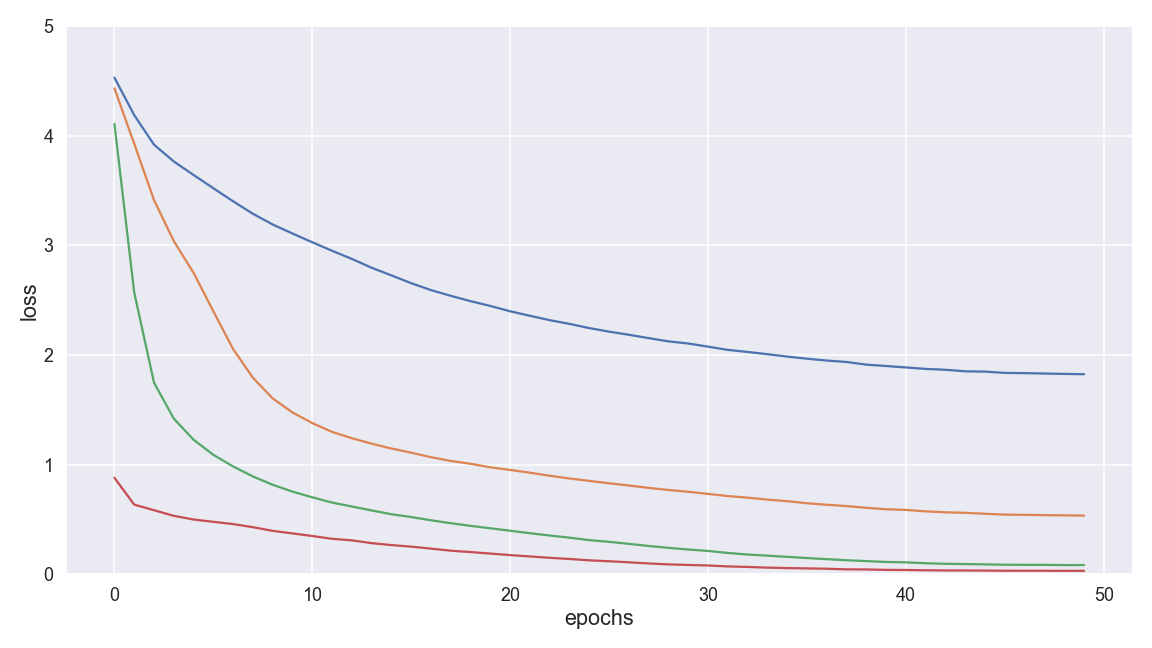
\includegraphics[width=.49\textwidth]{figures/training_plots/b-densenet_train-loss}}
	\subfloat[Test loss \label{fig:b-densenet-test-loss}]{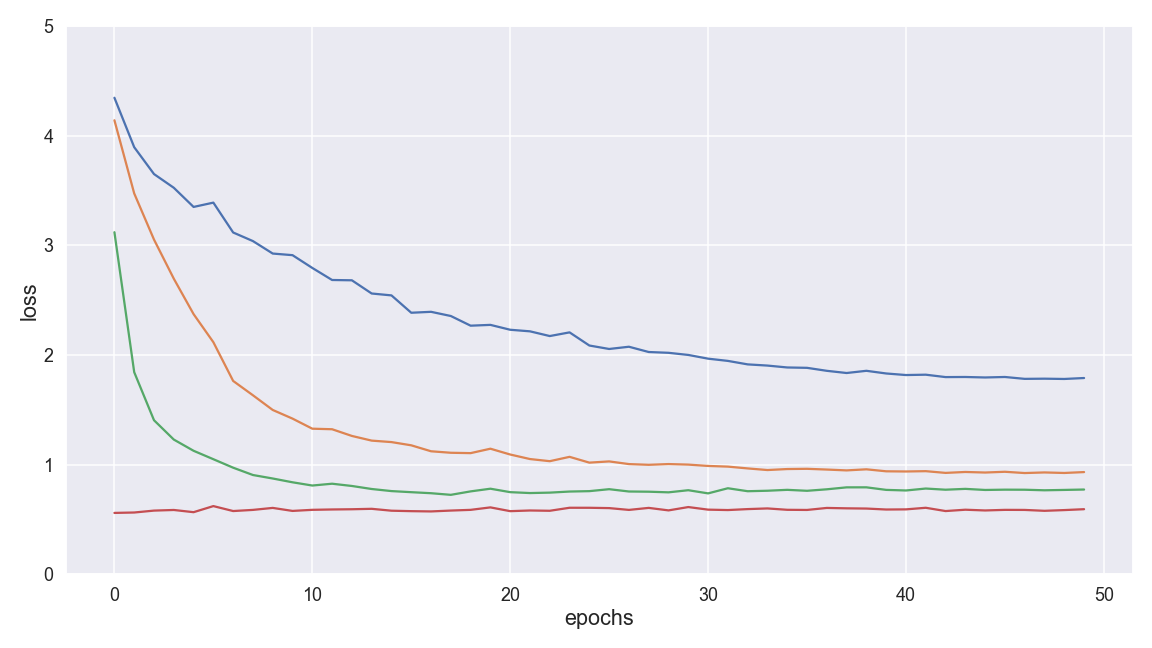
\includegraphics[width=.49\textwidth]{figures/training_plots/b-densenet_test-loss}}
	\hfill
	\subfloat[Train accuracy\label{fig:b-densenet-train-acc}]{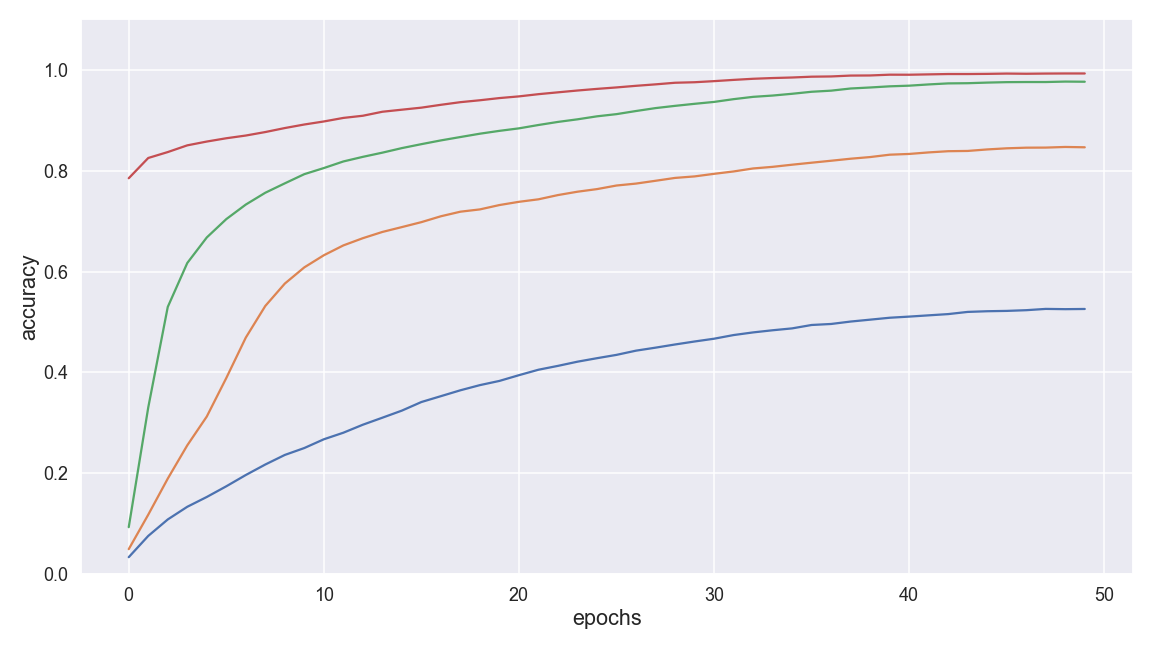
\includegraphics[width=.49\textwidth]{figures/training_plots/b-densenet_train-accuracy}}
	\subfloat[Test accuracy\label{fig:b-densenet-test-acc}]{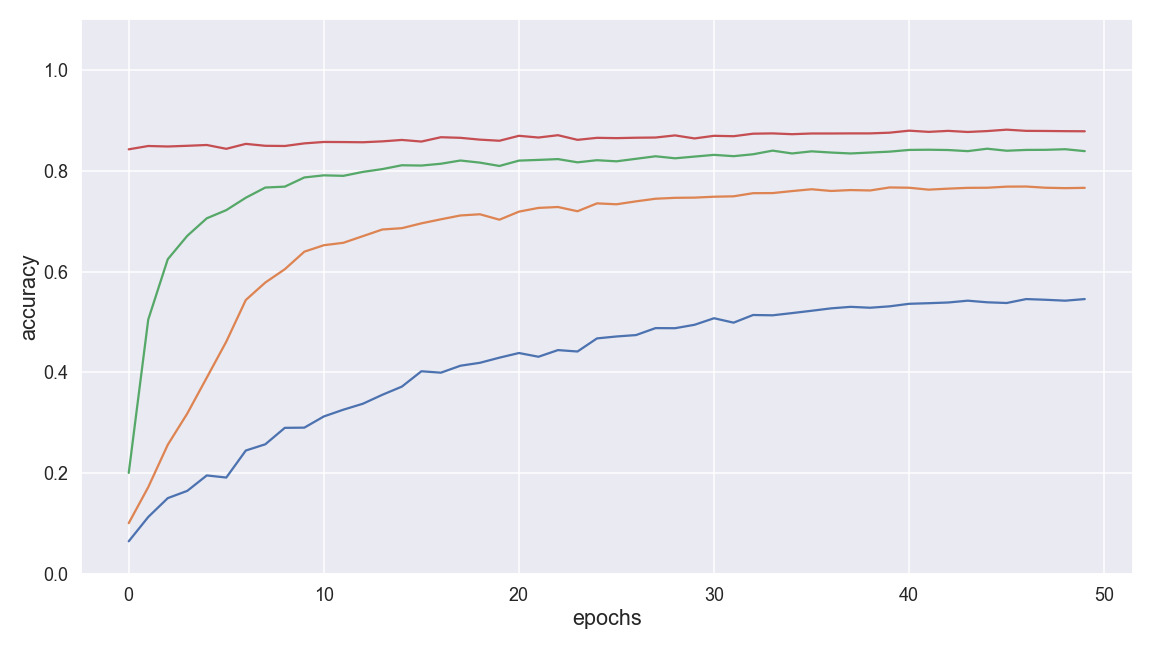
\includegraphics[width=.49\textwidth]{figures/training_plots/b-densenet_test-accuracy}}
	\caption[B-densenet Training summary]{B-densenet Training summary: shows the progression of model attributes over times of epochs, \protect\subref{fig:b-densenet-train-loss} train loss, \protect\subref{fig:b-densenet-test-loss} test loss, \protect\subref{fig:b-densenet-train-acc} train accuracy, \protect\subref{fig:b-densenet-test-acc}, test accuracy.}
	\label{fig:b-densenet-miniimagenet-100}
\end{figure}

Figure \ref{fig:msdnet-miniimagenet-100} show the results of training the \gls{msdnet}. The model specifically designed for early exiting shows indeed improvements for classifiers at early exit, but the overall accuracy i.e. the accuracy of the final classifier is slightly smaller compared to the other two models.

\begin{figure}
	\centering
	\captionsetup[subfigure]{justification=centering, farskip=1pt,captionskip=1pt}
	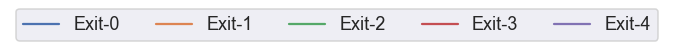
\includegraphics[width=.5\textwidth]{figures/training_plots/msdnet_exit_legend}
	\subfloat[Train loss\label{fig:msdnet-train-loss}]{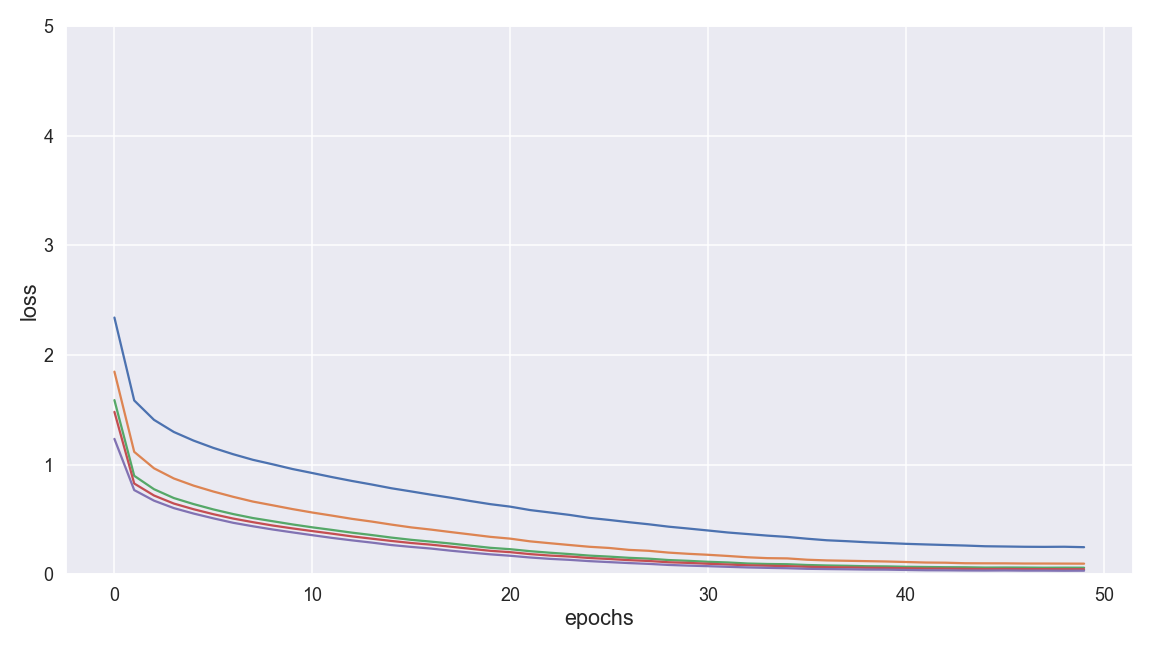
\includegraphics[width=.49\textwidth]{figures/training_plots/msdnet_train-loss}}
	\subfloat[Test loss \label{fig:msdnet-test-loss}]{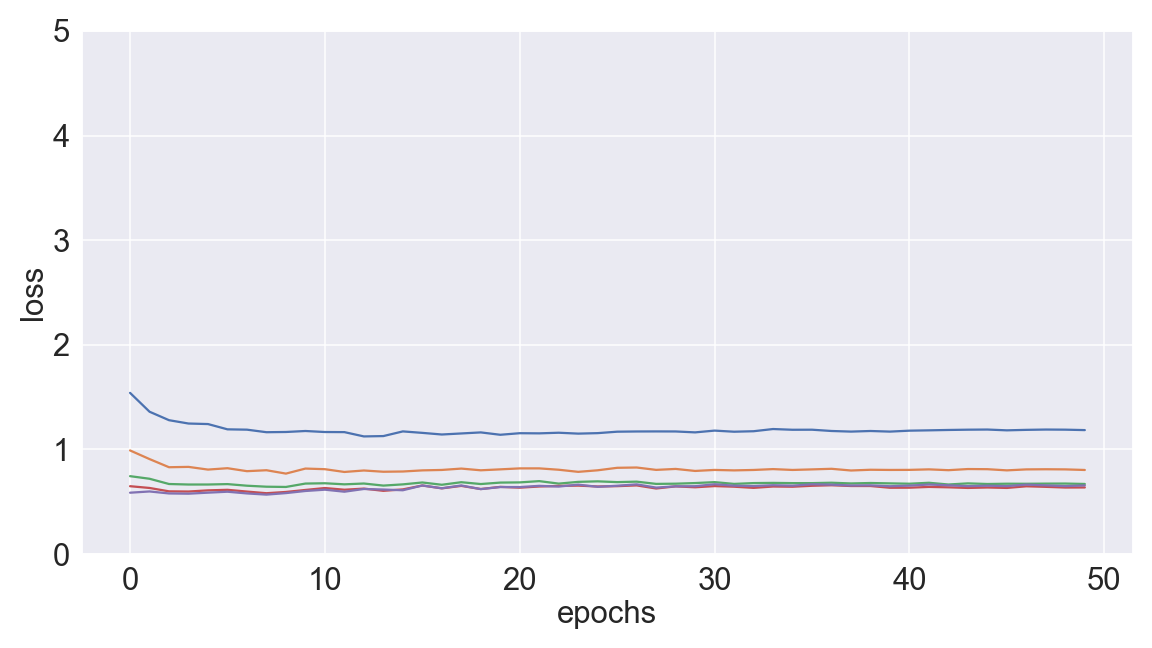
\includegraphics[width=.49\textwidth]{figures/training_plots/msdnet_test-loss}}
	\hfill
	\subfloat[Train accuracy\label{fig:msdnet-train-acc}]{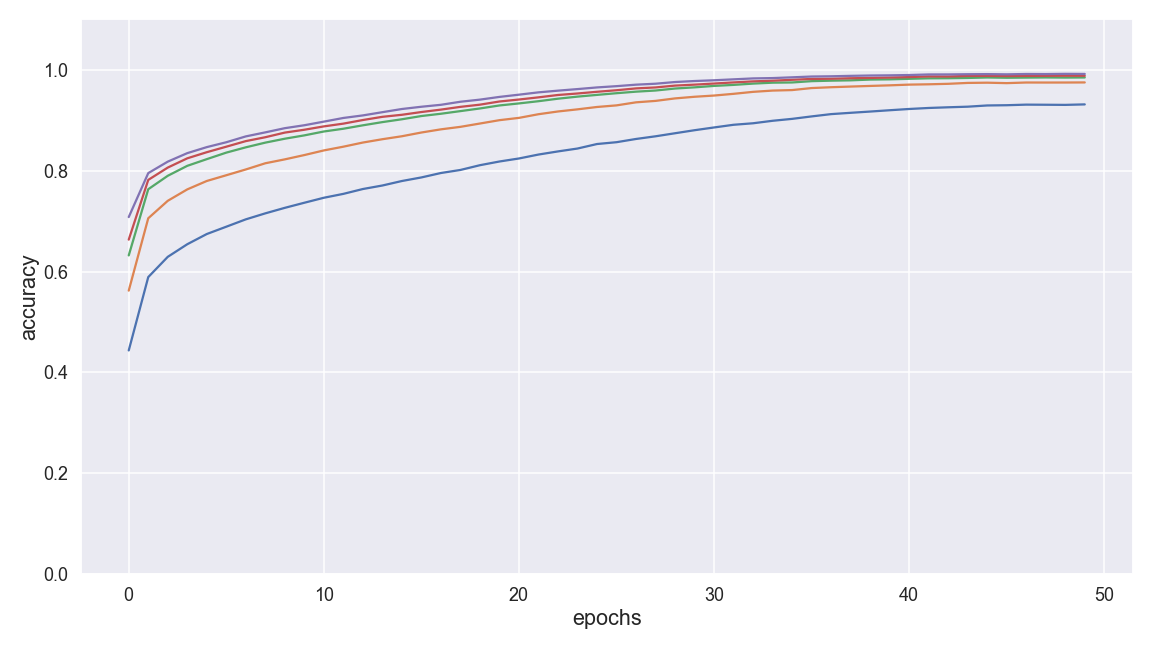
\includegraphics[width=.49\textwidth]{figures/training_plots/msdnet_train-accuracy}}
	\subfloat[Test accuracy\label{fig:msdnet-test-acc}]{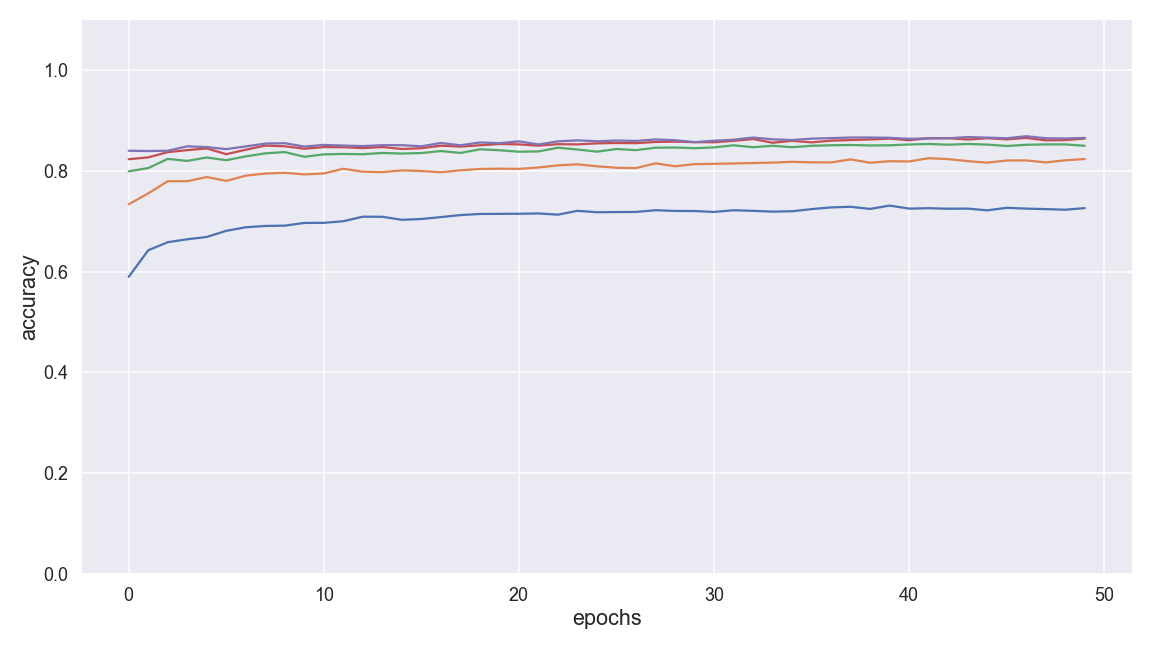
\includegraphics[width=.49\textwidth]{figures/training_plots/msdnet_test-accuracy}}
	\caption[MSDNet Training summary]{MSDNet Training summary: shows the progression of model attributes over times of epochs, \protect\subref{fig:msdnet-train-loss} train loss, \protect\subref{fig:msdnet-test-loss} test loss, \protect\subref{fig:msdnet-train-acc} train accuracy, \protect\subref{fig:msdnet-test-acc}, test accuracy.}
	\label{fig:msdnet-miniimagenet-100}
\end{figure}

Table \ref{tbl:training-compariosn} compares the best obtained validation accuracy in the training processes of the three models.


\begin{longtabu}{>{\bfseries}X[2]|X|X|X|X|X}
	\caption[Early Exiting Validation Accuracy from Training]{Early Exiting Validation Accuracy from Training} \label{tbl:training-compariosn} \\
	\toprule
	\rowfont{\bfseries}
	Model & Exit-0 & Exit-1 & Exit-2 & Exit-3 & Exit-4 \tabularnewline
	\bottomrule
	\endfirsthead
	\multicolumn{3}{@{}l}{\textbf{\textcolor{black}{Table \ref{tbl:frozen-vs-unfrozen}:}} continued}\\
	\toprule
	\rowfont{\bfseries}
	Model & Exit-0 & Exit-1 & Exit-2 & Exit-3 & Exit-4 \tabularnewline
	\bottomrule
	\endhead % all the lines above this will be repeated on every page
	\bottomrule
	\multicolumn{3}{@{}l}{continued \ldots}\\
	\endfoot
	\hline
	\endlastfoot
	B-\gls{resnet} & 0.49 	& 0.70 & 0.88 & 0.89 & N/A \tabularnewline
	\hline
	B-\gls{densenet}	& 0.55 	& 0.77 & 0.84 & 0.88 & N/A \tabularnewline
	\hline
	\gls{msdnet} & 0.73 & 0.82 & 0.85 &  0.87 & 0.87 \tabularnewline							
	\bottomrule
\end{longtabu}

In the next section we evaluate the trained models on the \gls{min100} validation set.

\subsection{Inference Results}

In this section we evaluate the accuracy of the early exit models. All validation samples are inferred to all model of table \ref{tbl:models}. Figure \ref{fig:exit-accuracy} show top-1 and top-5 accuracy of all exits of the three models.  

\begin{figure}
	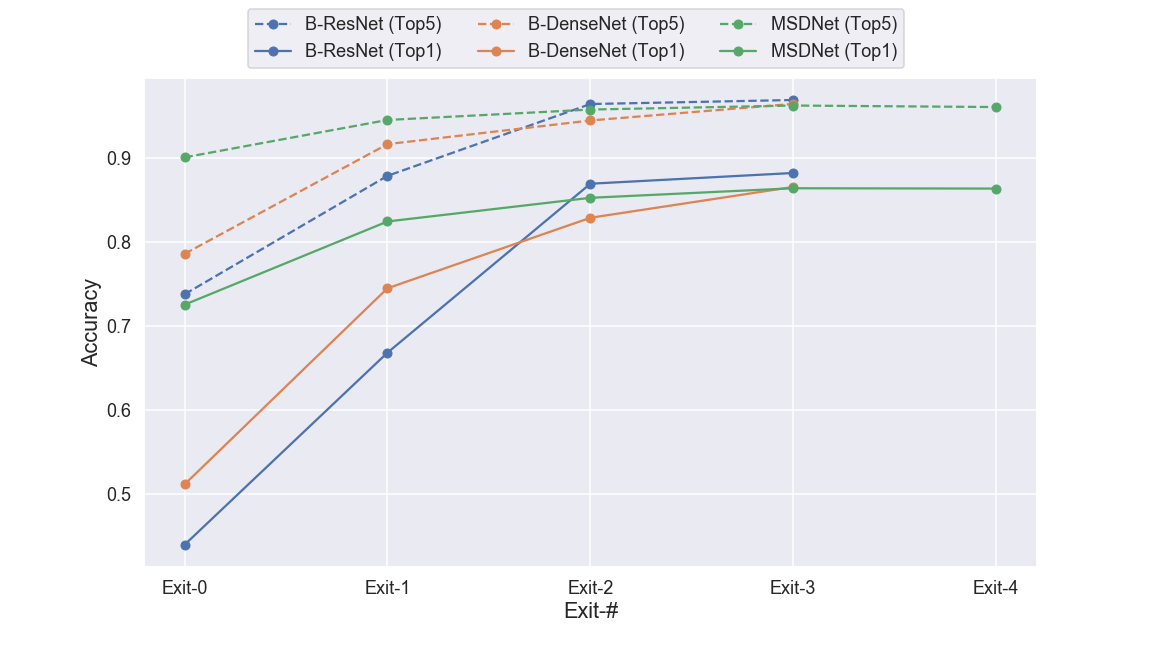
\includegraphics[width=\linewidth]{figures/inference_plots/accuracy-comparison}
	\caption[Accuracy of Early Exit Models]{Accuracy of Early Exit Models, B-\gls{resnet}, B-\gls{densenet} and \gls{msdnet}}
	\label{fig:exit-accuracy}
\end{figure}

As expected the models become more accurate, as the samples are predicted deeper in the network, as the increasingly complex features deep within the network have more discriminative characteristics. As stated in \cite{huang_multi-scale_2017} the densely connected features are important factors for obtaining intermediate classifiers with decent accuracy. The B-\gls{densenet} and \gls{msdnet} have as expected more accurate early classifiers, however the end-exit of B-\gls{resnet} achieves superior top-1 accuracy compared to the other models. Close to 50 \% of the samples can be accurately classified at the first exit of any of the model, which justifies the assumption for early exiting and promisingly, we should be able to save time. 

\subsubsection{Inference Time Analysis}

We setup a test, where we inference the entire \gls{min100} validation set the in all 5 models on three different platforms. Table \ref{tbl:inference-stats} show statistical values mean, standard deviation, minimum and maximum for the model inference time on the different platforms. From the table one can see, that the early exiting framework adds only a small additional delay, when comparing the last exit the \gls{branchynet} version with its conventional pendant. For the \gls{gpu}-enabled platforms, \gls{gpu} Workstation Jetson TX2, only additional 1.1ms and 2.4ms respectively on average. On the NUC the B-\gls{resnet} is 7.5 ms slower. 
\small{
\begin{longtabu}{>{\bfseries}X[2.6]|[1pt]X[r]|X[0.8r]|X[r]|X[1.2r]|[1pt]X[r]|X[0.7r]|X[r]|X[1.2r]|[1pt]X[r]|X[0.7r]|X[r]|X[1.2r]}
	\caption[Inference time statistics]{Inference time statistics (mean, standard deviation, minimum, maximum) of the five models on the three platforms }\label{tbl:inference-stats} \\
	\toprule
	\rowfont{\bfseries}
	& \multicolumn4{c|[1pt]}{GPU Workstation} &  \multicolumn4{c|[1pt]}{Jetson TX2} & \multicolumn4{c}{Intel NUC} \tabularnewline
	\tabucline{2-13}
	\rowfont{\bfseries} Model & Mean & Std.  & Min & Max & Mean & Std. & Min & Max & Mean & Std.  & Min & Max  \tabularnewline
	\hline
	\endfirsthead
	\multicolumn{3}{@{}l}{\textbf{\textcolor{black}{Table \ref{tbl:inference-stats}:}} continued}\\
	\toprule
	\rowfont{\bfseries}
	& \multicolumn4{c|[1pt]}{GPU Workstation} &  \multicolumn4{c|[1pt]}{Jetson TX2} & \multicolumn4{c}{Intel NUC} \tabularnewline
	\tabucline{2-13}
	\rowfont{\bfseries} Model & Mean & Std.  & Min & Max & Mean & Std.  & Min & Max & Mean & Std.  & Min & Max  \tabularnewline
	\hline
	\endhead % all the lines above this will be repeated on every page
	\hline
	\multicolumn{3}{@{}l}{continued \ldots}\\
	\endfoot
	\hline
	\endlastfoot
	ResNet  	& 36.01 & 1.72 & 33.24 & 69.02 & 64.19 & 1.95 & 61.28 & 110.17 & 215.76 & 21.98 & 132.98 & 275.55 \tabularnewline
	\hline
	DenseNet 	& 47.74 & 1.95 & 4.48 & 86.88 & 70.48 & 3.04 & 59.56 & 132.45 &  72.30 &  2.61 &  69.02 & 107.63 \tabularnewline
	\hline
	B-ResNet & & & &&&&&&&& &  \tabularnewline 
	\hspace{3mm} Exit-0 &  4.20 & 0.63 &  3.81 &  39.40 &  8.61 & 0.31 &  8.39 &  15.54 &  38.25 &  1.85 &  29.26 &  74.94 \tabularnewline
	\hspace{3mm} Exit-1 &  9.40 & 1.28 &  8.19 &  70.23 & 19.30 & 1.08 & 16.42 &  38.41 &  66.69 &  3.15 &  50.41 & 110.80 \tabularnewline
	\hspace{3mm} Exit-2 & 33.59 & 2.78 & 30.25 & 103.55 & 56.77 & 2.73 & 52.34 & 102.58 & 196.43 &  8.81 & 150.11 & 254.86 \tabularnewline
	\hspace{3mm} Exit-3 & 37.14 & 2.94 & 33.65 & 109.94 & 67.04 & 2.86 & 62.47 & 116.74 & 223.32 & 10.35 & 170.95 & 289.67 \tabularnewline
	\hline
	B-DenseNet &  & & &&&&&&&& & \tabularnewline
	\hspace{3mm} Exit-0 &  5.83 & 1.09 &  5.15 &  54.61 & 11.05 & 0.48 & 10.52 & 17.31 &  28.83 & 1.59 & 26.05 & 41.93 \tabularnewline
	\hspace{3mm} Exit-1 & 17.03 & 1.89 & 14.60 &  76.78 & 30.26 & 2.02 & 23.75 & 47.54 &  46.71 & 2.31 & 43.47 & 71.85 \tabularnewline
	\hspace{3mm} Exit-2 & 36.31 & 3.01 & 32.72 & 104.79 & 55.38 & 3.22 & 48.10 & 87.81 &  64.26 & 2.80 & 60.65 & 99.41 \tabularnewline
	\hspace{3mm} Exit-3 & 49.14 & 3.36 & 45.13 & 127.07 & 72.41 & 3.89 & 64.77 & 120.29 & 72.21 & 2.97 & 68.37 & 112.06 \tabularnewline
	\hline
	MSDNet & & &&&&&&&&&& \tabularnewline
	\hspace{3mm} Exit-0 & 24.14 & 1.59 & 21.53 &  67.38 &  40.37 & 2.77 & 29.36 & 209.89 & 19.99 & 1.27 & 16.99 &  35.12 \tabularnewline
	\hspace{3mm} Exit-1 & 42.24 & 2.54 & 38.87 & 119.85 &  65.18 & 4.29 & 53.34 & 267.19 & 32.82 & 2.38 & 29.03 & 103.19 \tabularnewline
	\hspace{3mm} Exit-2 & 55.59 & 2.82 & 51.90 & 143.30 &  83.81 & 5.43 & 71.39 & 312.55 & 42.89 & 3.03 & 38.72 & 130.52 \tabularnewline
	\hspace{3mm} Exit-3 & 64.49 & 2.99 & 60.59 & 156.26 &  96.53 & 6.26 & 83.68 & 345.67 & 50.10 & 3.43 & 45.66 & 145.75 \tabularnewline
	\hspace{3mm} Exit-4 & 68.87 & 3.11 & 64.85 & 165.90 & 103.29 & 6.65 & 90.14 & 361.02 & 56.02 & 3.62 & 51.28 & 154.08 \tabularnewline
	\bottomrule
\end{longtabu}}

Figure \ref{fig:inference-time-dist} shows the inference timing results as histograms. The inference time for each exit are plotted. The inference time are very different on the three platforms, and is very much dependent on the hardware characteristics, this is elaborated upon in section \ref{sec:ee-summary}.

\begin{figure}
	\begin{minipage}{\textwidth}
		\centering
		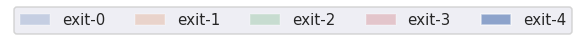
\includegraphics[width=.5\linewidth]{figures/inference_plots/time_dist_legend}
	\end{minipage}
	\begin{minipage}{0.33\textwidth}
		\captionsetup[subfigure]{farskip=0pt,captionskip=0pt, justification=centering}
		\centering
		GPU Workstation
		\subfloat[\gls{resnet} ]{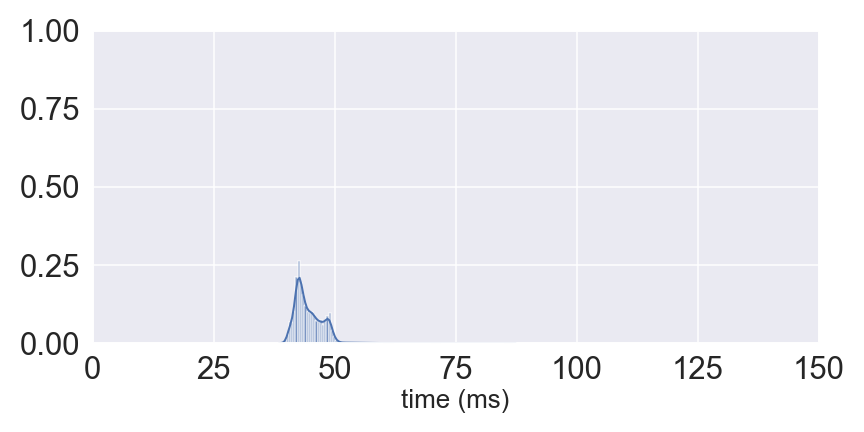
\includegraphics[width=\textwidth,height=.2\textheight,keepaspectratio]{figures/inference_plots/gpu_resnet_inference_time_distribution}}
		\hfill
		\subfloat[B-\gls{resnet}]{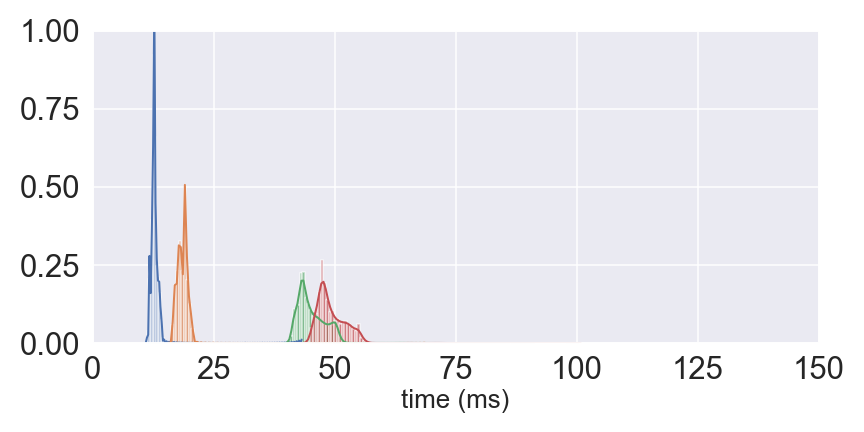
\includegraphics[width=\textwidth,height=.2\textheight,keepaspectratio]{figures/inference_plots/gpu_b-resnet_inference_time_distribution}}
		\hfill
		\subfloat[\gls{densenet} ]{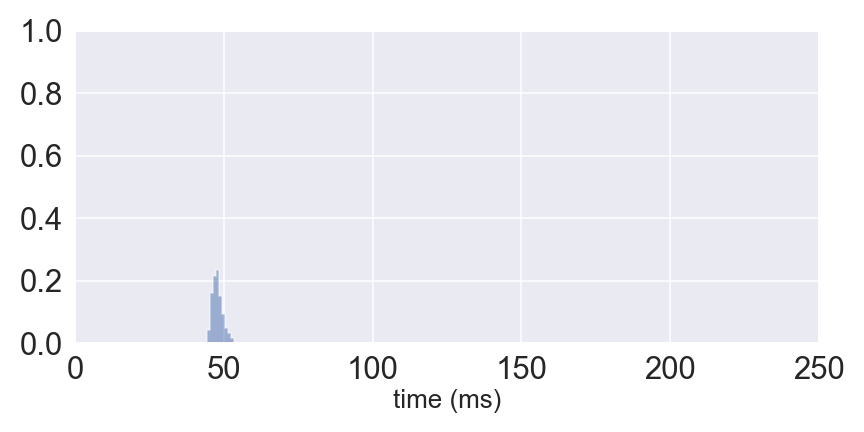
\includegraphics[width=\textwidth,height=.2\textheight,keepaspectratio]{figures/inference_plots/gpu_densenet_inference_time_distribution}}
		\hfill
		\subfloat[B-\gls{densenet}]{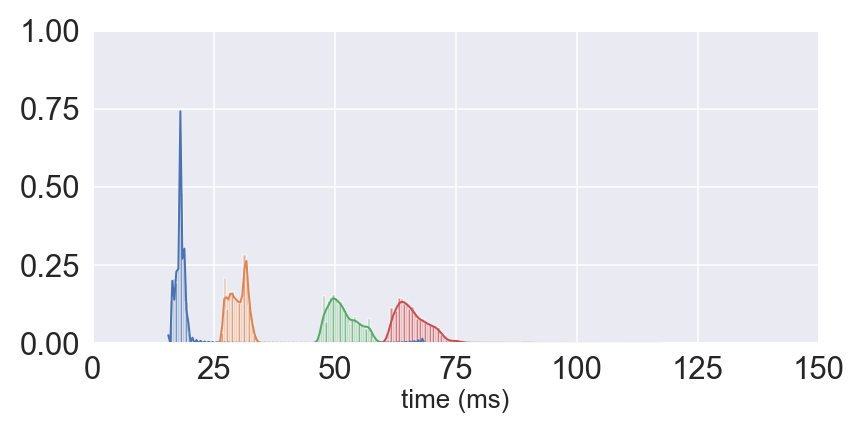
\includegraphics[width=\textwidth,height=.2\textheight,keepaspectratio]{figures/inference_plots/gpu_b-densenet_inference_time_distribution}}
		\hfill
		\subfloat[\gls{msdnet}]{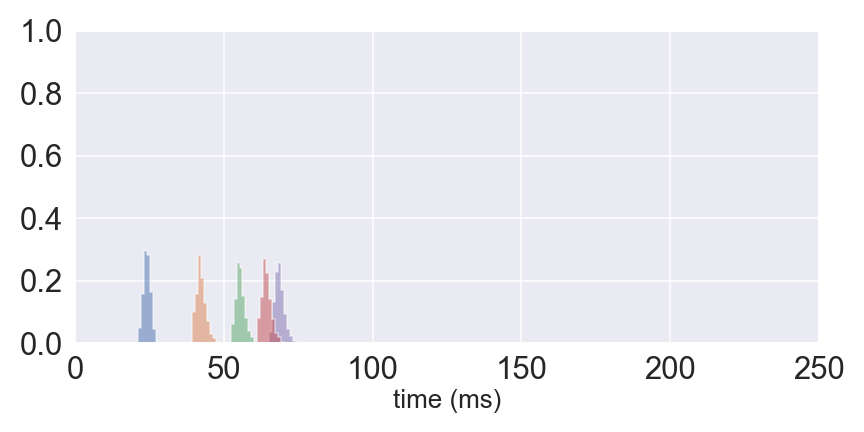
\includegraphics[width=\textwidth,height=.2\textheight,keepaspectratio]{figures/inference_plots/gpu_msdnet_inference_time_distribution}}
	\end{minipage}
	\begin{minipage}{0.33\textwidth}
		\captionsetup[subfigure]{farskip=0pt,captionskip=0pt,justification=centering}
		\centering
		Jetson TX2
		\subfloat[\gls{resnet} ]{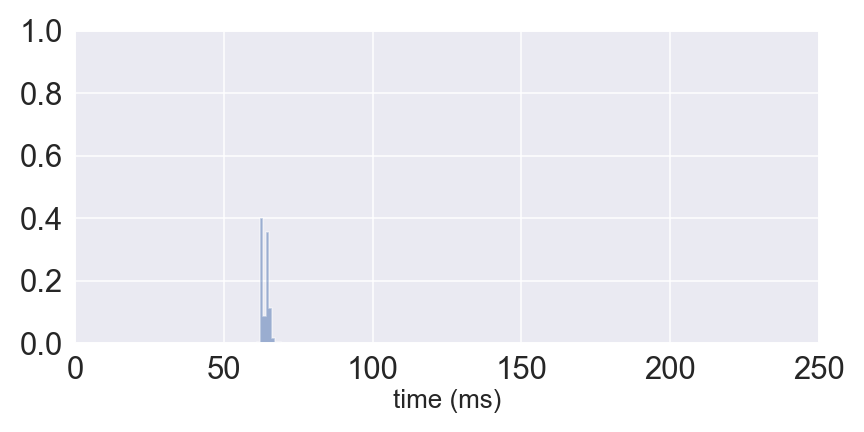
\includegraphics[width=\textwidth,height=.2\textheight,keepaspectratio]{figures/inference_plots/jetson_resnet_inference_time_distribution}}
		\hfill
		\subfloat[B-\gls{resnet}]{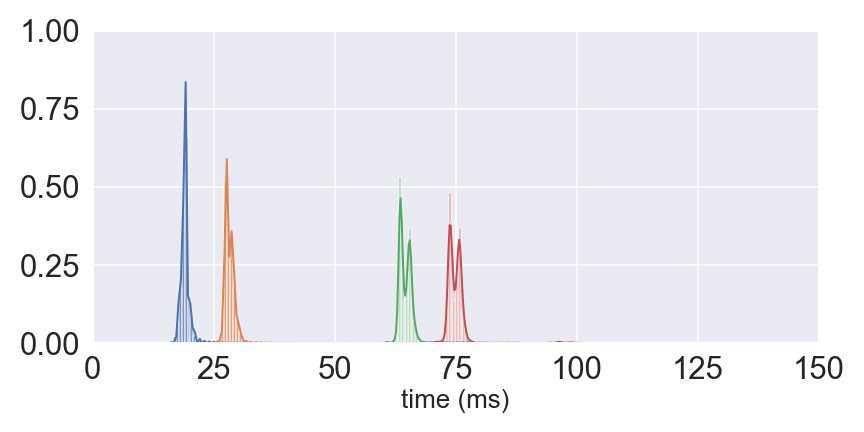
\includegraphics[width=\textwidth,height=.29\textheight,keepaspectratio]{figures/inference_plots/jetson_b-resnet_inference_time_distribution}}
		\hfill
		\subfloat[\gls{densenet} ]{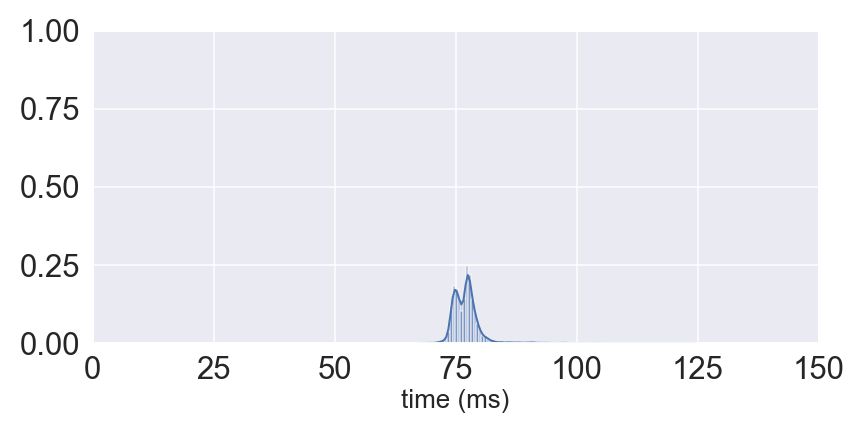
\includegraphics[width=\textwidth,height=.2\textheight,keepaspectratio]{figures/inference_plots/jetson_densenet_inference_time_distribution}}
		\hfill
		\subfloat[B-\gls{densenet}]{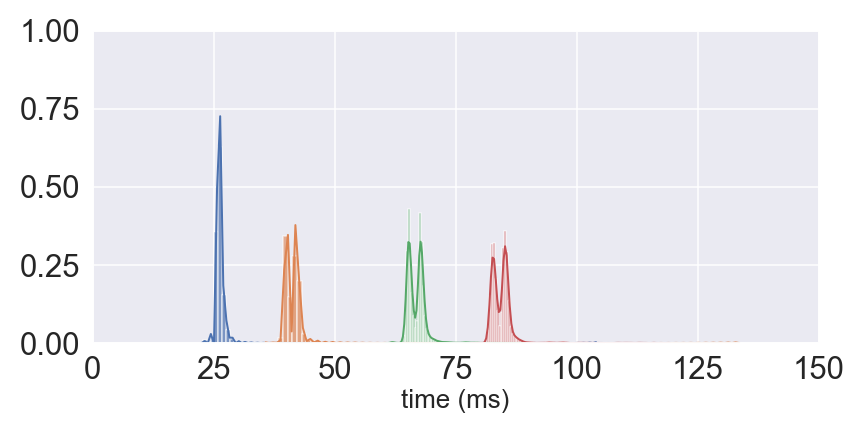
\includegraphics[width=\textwidth,height=.2\textheight,keepaspectratio]{figures/inference_plots/jetson_b-densenet_inference_time_distribution}}
		\hfill
		\subfloat[\gls{msdnet}]{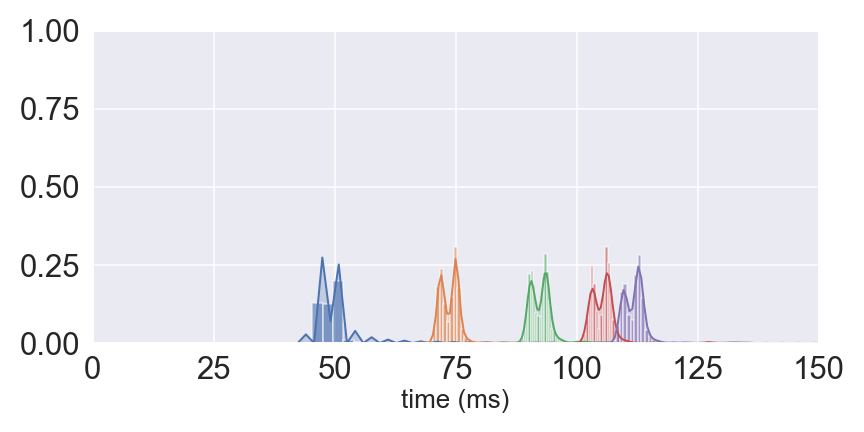
\includegraphics[width=\textwidth,height=.2\textheight,keepaspectratio]{figures/inference_plots/jetson_msdnet_inference_time_distribution}}
	\end{minipage}
	\begin{minipage}{.33\textwidth}
		\captionsetup[subfigure]{farskip=0pt,captionskip=0pt,justification=centering}
		\centering
		Intel NUC
		\subfloat[\gls{resnet} ]{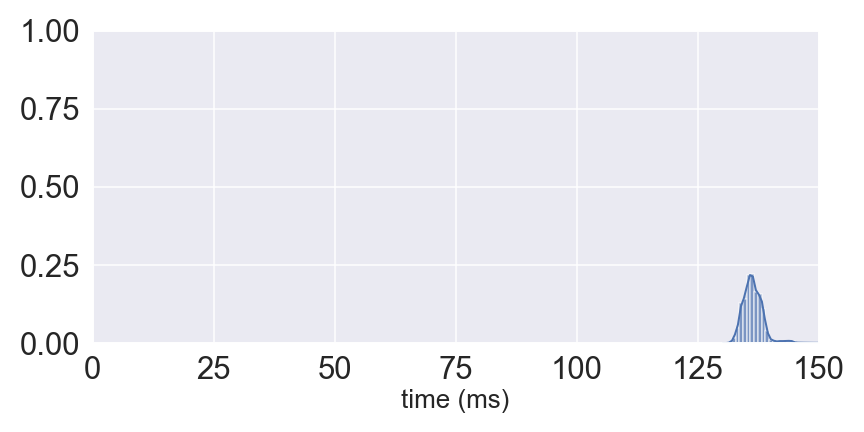
\includegraphics[width=\textwidth,keepaspectratio]{figures/inference_plots/nuc_resnet_inference_time_distribution}}
		\hfill
		\subfloat[B-\gls{resnet}]{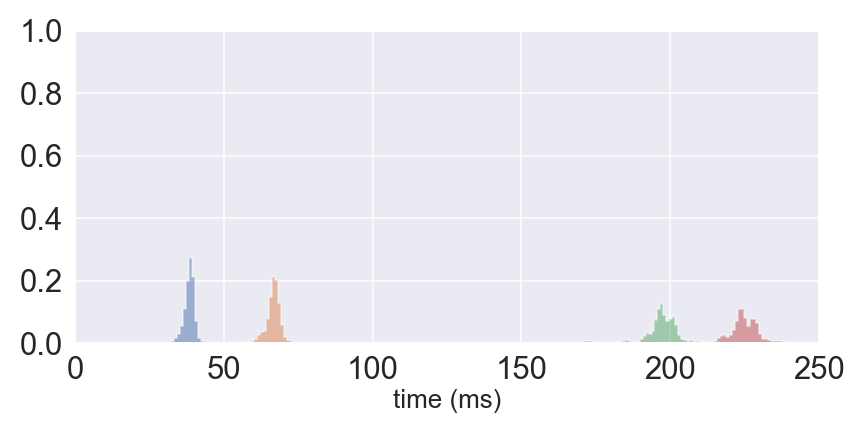
\includegraphics[width=\textwidth,height=.2\textheight,keepaspectratio]{figures/inference_plots/nuc_b-resnet_inference_time_distribution}}
		\hfill
		\subfloat[\gls{densenet} ]{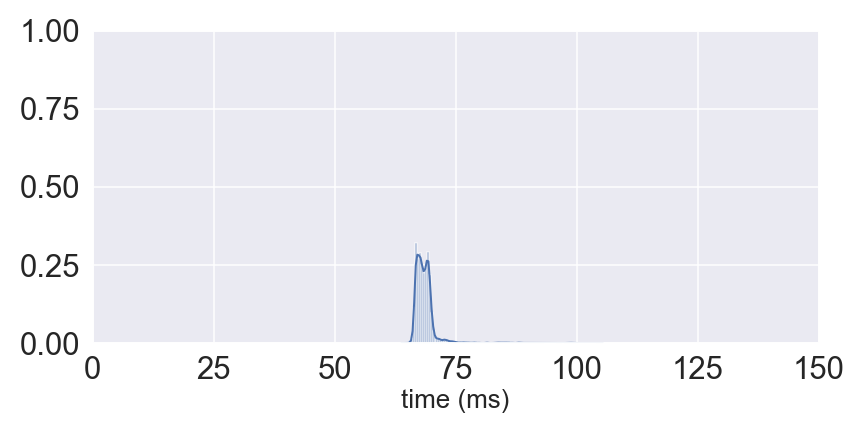
\includegraphics[width=\textwidth,keepaspectratio]{figures/inference_plots/nuc_densenet_inference_time_distribution}}
		\hfill
		\subfloat[B-\gls{densenet}]{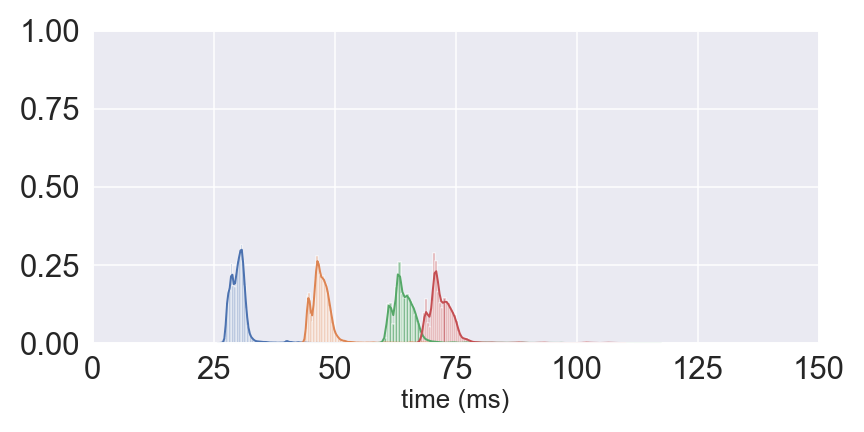
\includegraphics[width=\textwidth,keepaspectratio]{figures/inference_plots/nuc_b-densenet_inference_time_distribution}}
		\hfill
		\subfloat[\gls{msdnet}]{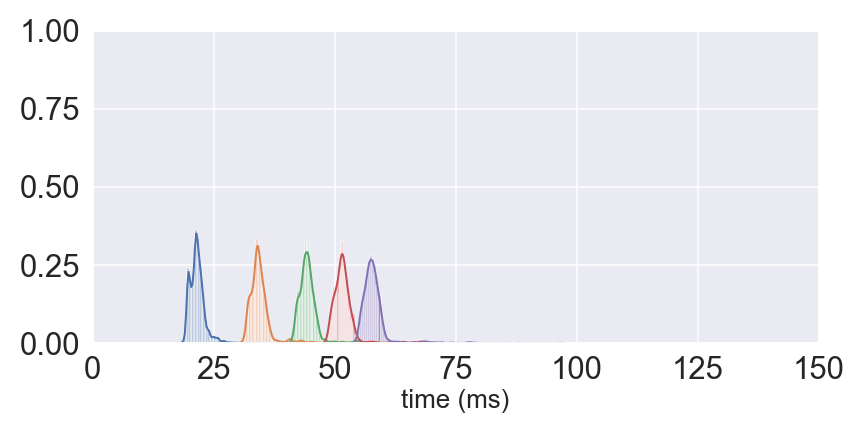
\includegraphics[width=\textwidth,keepaspectratio]{figures/inference_plots/nuc_msdnet_inference_time_distribution}}	
	\end{minipage}
	\caption[Platform Inference Time of \gls{dnn}s]{Inference Time Distribution, left column: GPU Workstation (a-e), center column: Jetson TX2 (f-j), right column NUC (k-o)}
	\label{fig:inference-time-dist}
\end{figure}

Still the challenge remains, how to determine when to let samples exit? As mentionend in section \ref{label}, it has been done in literature using a threshold measure of confidence \cite{leroux_cascading_2017, teerapittayanon_branchynet:_2016}. In the next section, we investigate how to allow samples to exit the model prematurely using the output from the softmax classfier. We experiment with two different scoring measures defined in section\ref{label}.


\subsubsection{Confidence Threshold Analysis}

Selecting threshold is a vital hyper-parameter for the accuracy-latency trade-off of early exiting models. If a too high threshold is selected only a few samples can confidently exit the model at an early exit, thus no significant delay improvements may be found. Contrary if too low a threshold is selected a huge delay improvement may be found, however at the cost of overall model accuracy. 

This analysis is theoretical, as the early exiting mechanism is in fact not exploited. All samples are allowed to pass all the way to the end of the network, thus all samples are classified at each exit, where both the prediction and score is logged. The prediction is evaluated against the ground truth and the score the two different score thrshold measures, \emph{Score-max} and \emph{Score-Margin}. If the score is higher than the threshold, the samples is marked as exited. \Cref{fig:resnet_confidence,fig:resnet_score-margin,fig:densenet_confidence,fig:densenet_score-margin,fig:msdnet_confidence,fig:msdnet_score-margin} compares the performance of each exit on all samples. The figures show for each of the early exit models under test. We plot the two thresholds score metrics for all exit of the models. The figures shows the frequency of exited samples, that have been correctly classified ({\color{sns-green}green}), and incorrectly classified samples, that the model have exited due to satisfying score ({\color{sns-red}red}). The samples, that could not be exited with proper confidence score given the magnitude of the threshold ({\color{sns-blue}blue}). The line plotted on each subfigure, shows the change in accuracy for the exit, as we raise the confidence score requirements ({\color{sns-orange}orange}).  

The aim is to find the metric, that reduces the amount of incorrectly exited samples ({\color{sns-red}red}). Whenever samples are exited incorrectly, the overall accuracy of the models are reduced, if it could have been correctly classifed at later exit. The growing frequency of correctly exited samples ({\color{sns-green}green}) at later exits, exemplifies exactly this improved accuracy at deeper layers of the models. As the value of the threshold are raised, it results in a higher accuracy for the exit, as the number incorrectly exited grows faster, than the number of correctly exited samples. 

Generally \emph{score-margin} has more desirable traits, as less samples are incorrectly exited ({\color{sns-red}red}), at the expense of additional samples not exited ({\color{sns-blue}blue}). \emph{Score-margin} is thus slower, but also more accurate, as fewer samples are incorrectly exited. The results matches \cite{park_big/little_2015}, which shows a stronger correlation between \emph{score-margin} and accuracy, than confidence score and accuracy.

We comparing the three models, we can see the impact of densely connected layer of B-\gls{densenet} and \gls{msdnet}, that are able to obtain higher scores at early exits, thus accurately exiting more samples prematurely. B-\gls{resnet} on the other hand are able to achieve higher end accuracy, as we did show in the section \ref{sec:early-exit-analysis}. The theoretical analysis is followed up by a practical test, where samples are exited if the threshold is passed. The test evaluates the threshold impact on accuracy and latency. 

\newcounter{imagenumber}
\begin{minipage}{\textwidth}
	\begin{figure}
		\centering
		\paragraph{B-ResNet}
		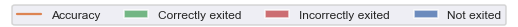
\includegraphics[width=\linewidth]{figures/threshold_plots/threshold_analysis_legend}
	\end{figure}
	
	\begin{minipage}{0.5\textwidth}
		\begin{figure}
			\captionsetup[subfloat]{farskip=1pt,captionskip=1pt, justification=centering}
			\centering
			\forloop{imagenumber}{0}{\value{imagenumber} < 4}{
				
				\subfloat[Exit-\arabic{imagenumber}\label{fig:confidence_resnet_exit_\arabic{imagenumber}}]{\includegraphics[width=.9\linewidth]{figures/threshold_plots/threshold_analysis_b-resnet_confidence_\arabic{imagenumber}}}
				\hfill
			}
			\caption[ResNet Confidence Threshold]{Confidence Threshold}
			\label{fig:resnet_confidence}
		\end{figure}
	\end{minipage}
	\begin{minipage}{0.5\textwidth}
		\begin{figure}
			\captionsetup[subfloat]{farskip=1pt,captionskip=1pt, justification=centering}
			\centering
			\forloop{imagenumber}{0}{\value{imagenumber} < 4}{
				
				\subfloat[Exit-\arabic{imagenumber}\label{fig:score-margin_resnet_exit_\arabic{imagenumber}}]{\includegraphics[width=.9\linewidth]{figures/threshold_plots/threshold_analysis_b-resnet_score-margin_\arabic{imagenumber}}}
				\hfill
			}
			\caption[ResNet Score-margin Threshold]{Score-margin Threshold}
			\label{fig:resnet_score-margin}
		\end{figure}
	\end{minipage}
\end{minipage}

\begin{minipage}{\textwidth}
	\begin{figure}
		\centering
		\paragraph{B-DenseNet}
	\end{figure}
	\begin{minipage}{0.5\textwidth}
		\begin{figure}
			\captionsetup[subfloat]{farskip=1pt,captionskip=1pt, justification=centering}
			\centering
			\forloop{imagenumber}{0}{\value{imagenumber} < 4}{
				
				\subfloat[Exit-\arabic{imagenumber}\label{fig:confidence_dense_exit_\arabic{imagenumber}}]{\includegraphics[width=.9\linewidth]{figures/threshold_plots/threshold_analysis_b-densenet_confidence_\arabic{imagenumber}}}
				\hfill
			}
			\caption[DenseNet Confidence Threshold]{Confidence Threshold}
			\label{fig:densenet_confidence}
		\end{figure}
	\end{minipage}
	\begin{minipage}{0.5\textwidth}
		\begin{figure}
			\captionsetup[subfloat]{farskip=1pt,captionskip=1pt, justification=centering}
			\centering
			\forloop{imagenumber}{0}{\value{imagenumber} < 4}{
				
				\subfloat[Exit-\arabic{imagenumber}\label{fig:score-dense_resnet_exit_\arabic{imagenumber}}]{\includegraphics[width=.9\linewidth]{figures/threshold_plots/threshold_analysis_b-densenet_score-margin_\arabic{imagenumber}}}
				\hfill
			}
			\caption[DenseNet Score-margin Threshold]{Score-margin Threshold}
			\label{fig:densenet_score-margin}
		\end{figure}
	\end{minipage}
\end{minipage}

\noindent\makebox[\textwidth][c]{\begin{minipage}{0.9\textwidth}
		\begingroup
		\leftskip=0cm plus 0.5fil \rightskip=0cm plus -0.5fil
		\parfillskip=0cm plus 1fil
		\paragraph{MSDNet}\par
		\endgroup
		
		\begin{minipage}{0.5\textwidth}
			\begin{figure}
				\captionsetup[subfloat]{farskip=0pt,captionskip=0pt, justification=centering}
				\centering
				\forloop{imagenumber}{0}{\value{imagenumber} < 5}{
					
					\subfloat[Exit-\arabic{imagenumber}\label{fig:confidence_msd_exit_\arabic{imagenumber}}]{\includegraphics[width=.9\linewidth]{figures/threshold_plots/threshold_analysis_msdnet_confidence_\arabic{imagenumber}}}
					\hfill
				}
				\caption[MSDNet Confidence Threshold]{Confidence Threshold}
				\label{fig:msdnet_confidence}
			\end{figure}
		\end{minipage}
		\begin{minipage}{0.5\textwidth}
			\begin{figure}
				\captionsetup[subfloat]{farskip=1pt,captionskip=1pt, justification=centering}
				\centering
				\forloop{imagenumber}{0}{\value{imagenumber} < 5}{
					
					\subfloat[Exit-\arabic{imagenumber}\label{fig:score-msdnet_exit_\arabic{imagenumber}}]{\includegraphics[width=.9\linewidth]{figures/threshold_plots/threshold_analysis_msdnet_score-margin_\arabic{imagenumber}}}
					\hfill
				}
				\caption[MSDNet Score-margin Threshold]{Score-margin Threshold}
				\label{fig:msdnet_score-margin}
			\end{figure}
		\end{minipage}
\end{minipage}}

\subsubsection{Practical Threshold Exiting}

We setup a test, where we use our three models, B-\gls{resnet}, B-\gls{densenet} and \gls{msdnet}. In this test a sample is exited when a threshold is passed, thus no additional prediction are tried for the sample, to evaluate early exiting capabilities in practice. If a samples reaches the last exit, it is classified irregardless of threshold being passed or not. Figure \ref{fig:model_c-threshold_comparison} presents the result using the score-max and figure \ref{fig:model_threshold_comparison} using the score-margin.

\begin{minipage}{\linewidth}
	\begin{figure}
		\captionsetup[subfloat]{justification=centering, captionskip=0pt, farskip=0pt}
		\centering
		\includegraphics[width=.5\linewidth]{figures/inference_plots/model_bar_legend}
	\end{figure}
	\begin{figure}
		\captionsetup[subfloat]{justification=centering, captionskip=0pt, farskip=1pt}
		\centering
		\subfloat[$T= 0.1$\label{fig:model-c-threshold_comparison_t_1}]{\includegraphics[width=.33\linewidth]{figures/inference_plots/model_confidence_comparison_1}}
		\hfill
		\subfloat[$T= 0.2$\label{fig:model-c-threshold_comparison_t_2}]{\includegraphics[width=.33\linewidth]{figures/inference_plots/model_confidence_comparison_2}}
		\hfill
		\subfloat[$T= 0.3$\label{fig:model-c-threshold_comparison_t_3}]{\includegraphics[width=.33\linewidth]{figures/inference_plots/model_confidence_comparison_3}}
		\hfill
		\subfloat[$T= 0.4$\label{fig:model-c-threshold_comparison_t_4}]{\includegraphics[width=.33\linewidth]{figures/inference_plots/model_confidence_comparison_4}}
		\hfill
		\subfloat[$T= 0.5$\label{fig:model-c-threshold_comparison_t_5}]{\includegraphics[width=.33\linewidth]{figures/inference_plots/model_confidence_comparison_5}}
		\hfill
		\subfloat[$T= 0.6$\label{fig:model-c-threshold_comparison_t_6}]{\includegraphics[width=.33\linewidth]{figures/inference_plots/model_confidence_comparison_6}}
		\hfill
		\subfloat[$T= 0.7$\label{fig:model-c-threshold_comparison_t_7}]{\includegraphics[width=.33\linewidth]{figures/inference_plots/model_confidence_comparison_7}}
		\hfill
		\subfloat[$T= 0.8$\label{fig:model-c-threshold_comparison_t_8}]{\includegraphics[width=.33\linewidth]{figures/inference_plots/model_confidence_comparison_8}}
		\hfill
		\subfloat[$T= 0.9$\label{fig:model-c-threshold_comparison_t_9}]{\includegraphics[width=.33\linewidth]{figures/inference_plots/model_confidence_comparison_9}}
		
		\caption[Model comparison of early exit capabilities using confidence threshold]{Model comparison of early exit capabilities using score-max}
		\label{fig:model_c-threshold_comparison}
	\end{figure}
	
\end{minipage}

\begin{minipage}{\linewidth}
	\begin{figure}
		\captionsetup[subfloat]{justification=centering, captionskip=0pt, farskip=0pt}
		\centering
		\includegraphics[width=.5\linewidth]{figures/inference_plots/model_bar_legend}
	\end{figure}
	\begin{figure}
		\captionsetup[subfloat]{justification=centering, captionskip=0pt, farskip=1pt}
		\centering
		\subfloat[$T= 0.1$\label{fig:model-threshold_comparison_t_1}]{\includegraphics[width=.33\linewidth]{figures/inference_plots/model_comparison_1}}
		\hfill
		\subfloat[$T= 0.2$\label{fig:model-threshold_comparison_t_2}]{\includegraphics[width=.33\linewidth]{figures/inference_plots/model_comparison_2}}
		\hfill
		\subfloat[$T= 0.3$\label{fig:model-threshold_comparison_t_3}]{\includegraphics[width=.33\linewidth]{figures/inference_plots/model_comparison_3}}
		\hfill
		\subfloat[$T= 0.4$\label{fig:model-threshold_comparison_t_4}]{\includegraphics[width=.33\linewidth]{figures/inference_plots/model_comparison_4}}
		\hfill
		\subfloat[$T= 0.5$\label{fig:model-threshold_comparison_t_5}]{\includegraphics[width=.33\linewidth]{figures/inference_plots/model_comparison_5}}
		\hfill
		\subfloat[$T= 0.6$\label{fig:model-threshold_comparison_t_6}]{\includegraphics[width=.33\linewidth]{figures/inference_plots/model_comparison_6}}
		\hfill
		\subfloat[$T= 0.7$\label{fig:model-threshold_comparison_t_7}]{\includegraphics[width=.33\linewidth]{figures/inference_plots/model_comparison_7}}
		\hfill
		\subfloat[$T= 0.8$\label{fig:model-threshold_comparison_t_8}]{\includegraphics[width=.33\linewidth]{figures/inference_plots/model_comparison_8}}
		\hfill
		\subfloat[$T= 0.9$\label{fig:model-threshold_comparison_t_9}]{\includegraphics[width=.33\linewidth]{figures/inference_plots/model_comparison_9}}
		
		\caption[Model comparison of early exit capabilities]{Model comparison of early exit capabilities using score-margin}
		\label{fig:model_threshold_comparison}
	\end{figure}
	
\end{minipage}

The subfigures of figure \ref{fig:model_c-threshold_comparison} and \ref{fig:model_threshold_comparison} show the raised score requirements. Each subfigure presents a subplot of the frequency of correctly exited samples and a subplot of incorrectly exit samples at each exit for all three models. Note, for each model i.e. same colored bars sum to one across the subplot, which is equivalent to all samples of the test. From the figures we can tell, that less samples are incorrect classified, as we select a higher threshold and thus forcing the model to use later exits. B-\gls{densenet} and especially \gls{msdnet} designed for early-exiting, are able to more frequently exit samples at early exits even at low thresholds values. Given this insight we use timings from the test to evaluate threshold impact on the accuracy-latency trade-off.

%\subsubsection{Accuracy-Latency Trade-Off Analysis}

Figure \ref{fig:threshold-acc-lat-trade-off} show the inference accuracy and latency on the three different platforms. Irregardless of platform, the results clearly exemplifies the accuracy-latency trade-off imposed by the early exit model. As we raise the score requirements, we improve the models' accuracy, however we introduce more latency, as we enforce the frequency of samples, requiring a later exit to reach a satisfying score, to grow. 



% B-\gls{densenet} benefits more from early exiting, when a threshold of 0.9 is chosen, it gives up 4 percentage point in accuracy and reducing inference latency by 29 \%. The B-\gls{resnet} have about the same compromise in terms of accuracy, however only a reduction of 18 \% inference latency. B-\gls{resnet} still perform better in terms of both accuracy and inference time on the \gls{gpu}-enabled devices.


\begin{figure}
	\captionsetup[subfigure]{justification=centering,farskip=0pt,captionskip=0pt}
	\centering
	\includegraphics[width=.4\linewidth]{figures/threshold_plots/inference_legend}
	\subfloat[GPU Workstation\label{fig:early_exit_vs_conv}]{\includegraphics[width=\textwidth,height=.22\textheight,keepaspectratio]{figures/threshold_plots/gpu_inference}}
	\hfill
	\subfloat[Jetson TX2\label{fig:jetson-early_exit_vs_conv}]{\includegraphics[width=\textwidth,height=.22\textheight,keepaspectratio]{figures/threshold_plots/jetson_inference}}
	\hfill
	\subfloat[NUC\label{fig:nuc-early_exit_vs_conv}]{\includegraphics[width=\textwidth,height=.22\textheight,keepaspectratio]{figures/threshold_plots/nuc_inference}}
	\caption[Threshold Accuracy-Latency Trade-off]{Threshold Accuracy-Latency Trade-off on \protect\subref{fig:early_exit_vs_conv} GPU Workstation, \protect\subref{fig:jetson-early_exit_vs_conv} Jetson TX2 and \protect\subref{fig:nuc-early_exit_vs_conv} NUC }
	\label{fig:threshold-acc-lat-trade-off}
\end{figure}

In figure \ref{fig:threshold-acc-lat-trade-off-by-time} we combine the subplot of figure \ref{fig:threshold-acc-lat-trade-off}, by plotting the accuracy against the mean time. The figure makes it easier tom compare the accuracy-latency trade-off. The conventional models are clearly more accurate, however also expectantly slower, than their more flexible exiting counterpart. B-\gls{resnet} is the best model on the \gls{gpu}-workstation and the Jetson. On the NUC, we can see B-\gls{resnet} requires much time to outperform the other two, where \gls{msdnet} is outstanding the best model. 

\begin{figure}
	\captionsetup[subfigure]{justification=centering,farskip=0pt,captionskip=0pt}
	\centering
	\includegraphics[width=.4\linewidth]{figures/threshold_plots/inference_by_time_legend}
	\subfloat[GPU Workstation\label{fig:gpu-early_exit_vs_time}]{\includegraphics[width=\textwidth,height=.22\textheight,keepaspectratio]{figures/threshold_plots/gpu_inference_by_time}}
	\hfill
	\subfloat[Jetson TX2\label{fig:jetson-early_exit_vs_time}]{\includegraphics[width=\textwidth,height=.22\textheight,keepaspectratio]{figures/threshold_plots/jetson_inference_by_time}}
	\hfill
	\subfloat[NUC\label{fig:nuc-early_exit_vs_time}]{\includegraphics[width=\textwidth,height=.22\textheight,keepaspectratio]{figures/threshold_plots/nuc_inference_by_time}}
	\caption[Threshold Accuracy-Latency Trade-off]{Threshold Accuracy-Latency Trade-off on \protect\subref{fig:early_exit_vs_conv} GPU Workstation, \protect\subref{fig:jetson-early_exit_vs_conv} Jetson TX2 and \protect\subref{fig:nuc-early_exit_vs_conv} NUC }
	\label{fig:threshold-acc-lat-trade-off-by-time}
\end{figure}

We have shown, that early exit model can be used to reduce the latency with a compromise in accuracy, adjusted by a score threshold. The question, that remains is still, can we use early exits to meet delay requirement for time-critical application. 

\subsubsection{Delay Threshold Analysis}

We setup another test to evaluate early exit model for time-critical applications. Having a time-budget sets a different requirement, that a prediction must be acquired before a deadline. As defined in equation \ref{label}, we want to maximize the accuracy subject to this time constraint. In the test we inference the validation samples to all model on all platforms. We measure the time to reach a prediction at all exits of the model. We plot, in figure \ref{fig:delay-threshold}, the reliability (eq. \ref{label}) against delay thresholds.

\begin{figure}
	\captionsetup[subfigure]{justification=centering, farskip=0pt,captionskip=0pt}
	\centering
	\includegraphics[height=.05\textheight]{figures/delay_plots/delay_threshold_legend}
	\hfill
	\subfloat[GPU Workstation]{\includegraphics[width=\textwidth,height=.22\textheight,keepaspectratio]{figures/delay_plots/gpu__delay_threshold}}
	\hfill
	\subfloat[Jetson TX2]{\includegraphics[width=\textwidth,height=.22\textheight,keepaspectratio]{figures/delay_plots/jetson__delay_threshold}}
	\hfill
	\subfloat[NUC]{\includegraphics[width=\textwidth,height=.22\textheight,keepaspectratio]{figures/delay_plots/nuc__delay_threshold}}
	\caption[Delay Threshold]{Time Threshold}
	\label{fig:delay-threshold}
\end{figure}

The result show staircase-like functions of reliability as we relax the delay constraint, which increases the reliability when more time ia available. The steps of the functions are loacted close to the mean time-to-prediction for a later exit of the model, see table \ref{label}. The dashed lines show the conventional model, clearly under very stringent delay requirement, we are able to improve the reliability using early exit models. However, if the last exit of the early exit model is always reachable, then the conventional models achieve superior reliability. 

In the next section, we summarize, discuss and conclude our findings of investigating the early exit model capabilities in this chapter. In the next chapter we use early exiting in edge offloading scenarios to improve the reliability of time-critical applicaitons at the edge.

\section{Summary} \label{sec:ee-summary}

To summarize this chapter about the early exit \gls{dnn}, we have successfully trained three early exiting models on the \gls{min100} dataset. We did show, that freezing the model base, did not allow for features to be optimized the classifiers at early exits. Training the entire model, on the other hand did show satisfying validation accuracy. The \gls{msdnet} is able to obtain the best accuracy on the early exits, but B-\gls{resnet} is able to obtain higher accuracy at the final exit. 

We measured inference time on three hardware platforms, which gave very different results. The inference timings are dependent on the hardware characteristics. The GPU Workstation are enabled with the strongest \gls{gpu}, thus have the most parallelization capabilities and able to run \gls{resnet} faster, as it requires enormous amounts of \gls{flop}s well-suited for \gls{gpu} acceleration. \gls{densenet} and \gls{msdnet} has much lower amount of parameter and required musch less \gls{flop}s and would be expected to run faster. However, the densely connected block uses concatenation which might be a more expensive operation on the \gls{gpu}. The Intel NUC, shows the opposite trend, in fact the \gls{msdnet} outperform the other models, as it requires far fewer G\gls{flop}s and are comprised of far fewer layers and parameters. The \gls{cpu}-only NUC cannot achieve the same level of parallelization to accelerate model inference.

We investigated confidence threshold as a measure to exit samples prematurely. We used both score-max and score-margin. The score-margin was able to remove most incorrectly exited samples, when choosing a sufficiently high threshold value. However, it was at the cost of some samples, that could have exited correctly, now not able to be exited. Additionally we compared the early exiting capabilities of the models. The model comprised of densely connected blocks B-\gls{densenet} and \gls{msdnet}, was able to correctly exit more sample at early exits, where the model designed for early exiting, \gls{msdnet} outperformed its competitor. We also studied the accuracy-latency trade-off, by letting samples exit the model at early exits. Early exit models can indeed save time compared with the conventional models, especially when selecting a low threshold value. Only if selecting 1 as threshold value will the early exit model be slower, than its conventional counterpart. We compared the models by plotting the accuracy by time, the B-\gls{resnet} was found out to be the best model at making a compromise between accuracy and latency on the \gls{gpu}-enabled platforms. In sharp contrast to the \gls{cpu} of the NUC, where both the B-\gls{densenet} and \gls{msdnet} were better.

Finally, we evaluated the obtainable accuracy by a delay threshold. The conventional models are outperformed at stringent delay threshold. B-\gls{resnet} is still the better on the \gls{gpu}-enabled platforms. However, not as exclusively as figure \ref{fig:threshold-acc-lat-trade-off-by-time} shows. At certain delay threshold B-\gls{densenet} is actually better. Figure \ref{fig:delay-threshold} encourages a model selection, where the most accurate model is chosen based on the required delay threshold. 

All analyses have led us to a scheme suitable for edge offloading, which is explained in the next chapter.
